\documentclass[a4paper]{ltjsarticle}

\usepackage[margin=15mm]{geometry}

\usepackage{graphicx}
\usepackage{makeidx}
\usepackage[font=current]{idxlayout}
\makeindex

\begin{document}

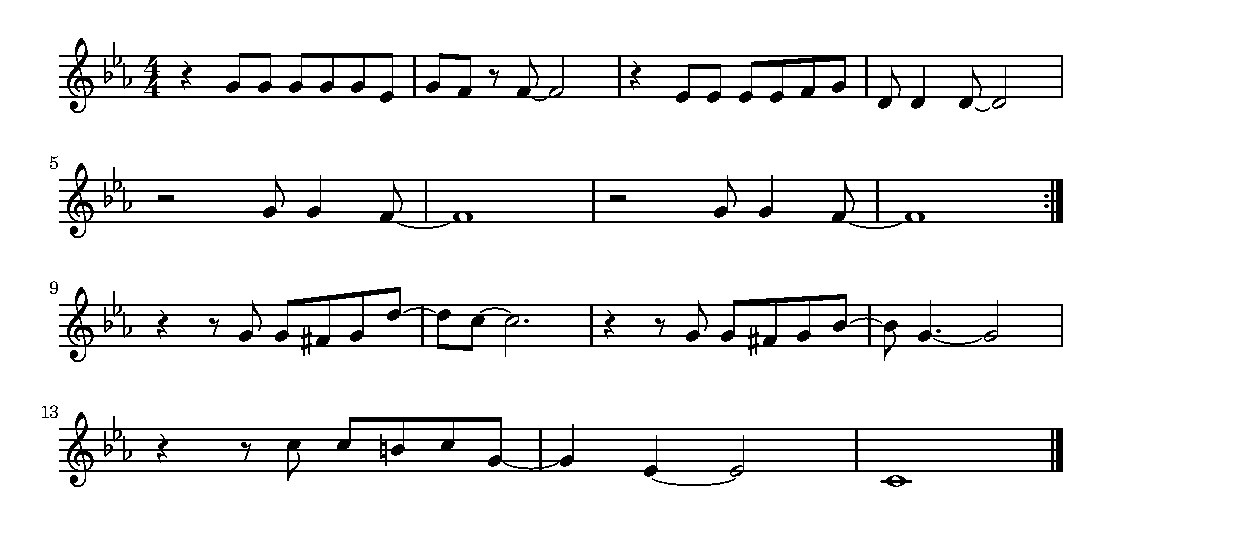
\includegraphics[clip]{christmaseve_crop.pdf}

\vspace{-10mm} \hspace{10mm}
クリスマス・イブ(きっとあなたはこない、山下達郎)
\index{くりすます@クリスマス・イブ(きっとあなたはこない、山下達郎)}

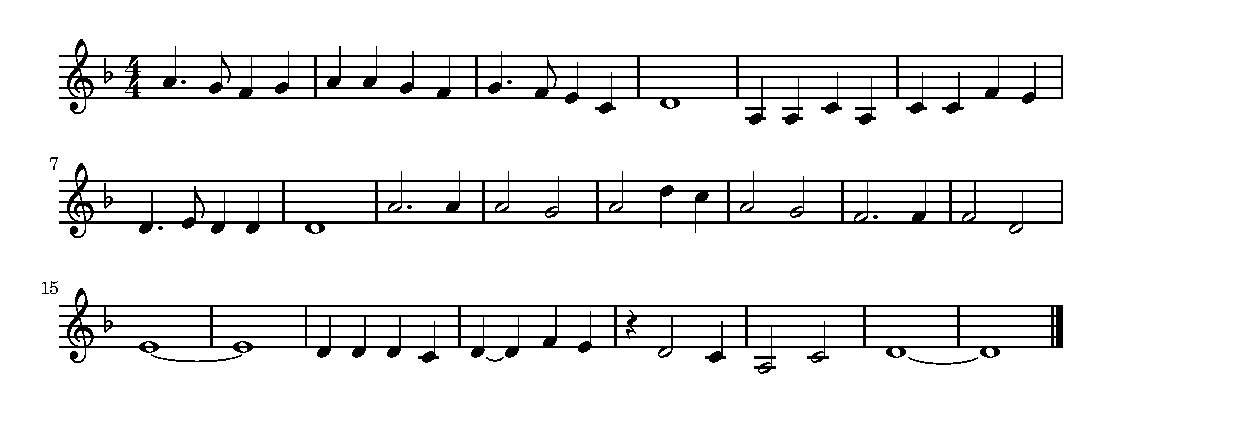
\includegraphics[clip]{mitokomon_crop.pdf}

\vspace{-10mm} \hspace{10mm}
水戸黄門(じんせいらくありゃくもあるさ)
\index{みとこうもん@水戸黄門(じんせいらくありゃくもあるさ)}

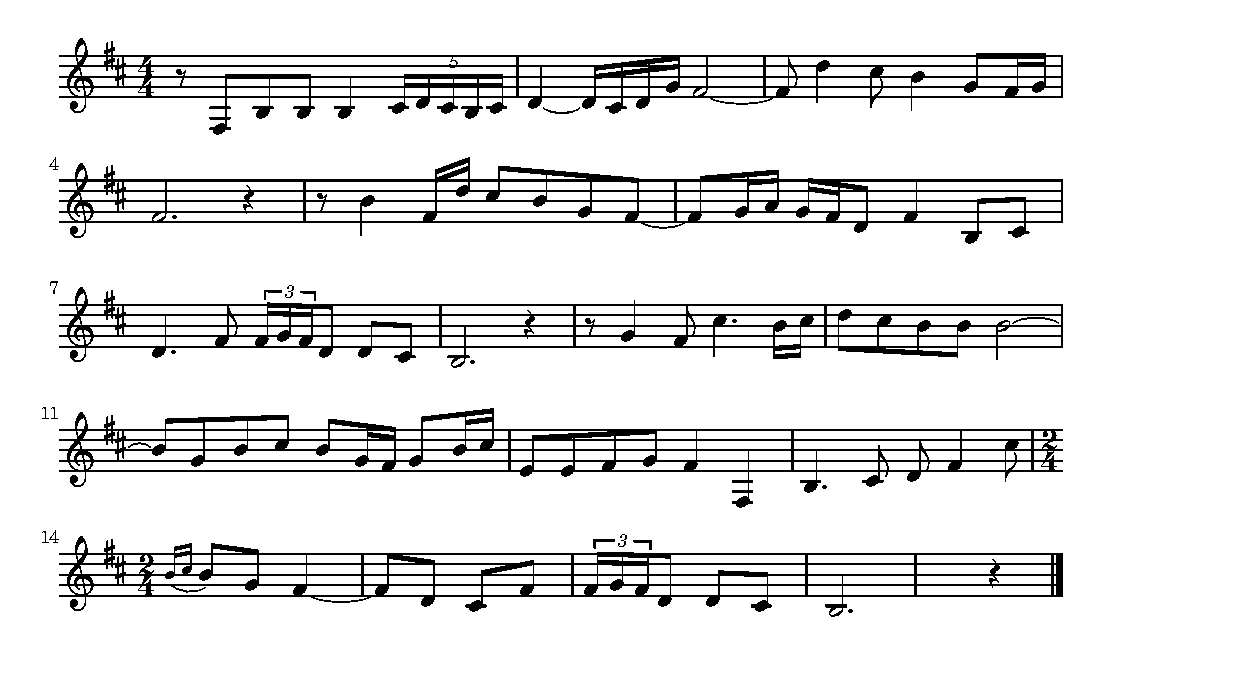
\includegraphics[clip]{yunomachielegy_crop.pdf}

\vspace{-10mm} \hspace{10mm}
湯の町エレジー(いずのやまやまつきあわく)
\index{ゆのまち@湯の町エレジー(いずのやまやまつきあわく)}

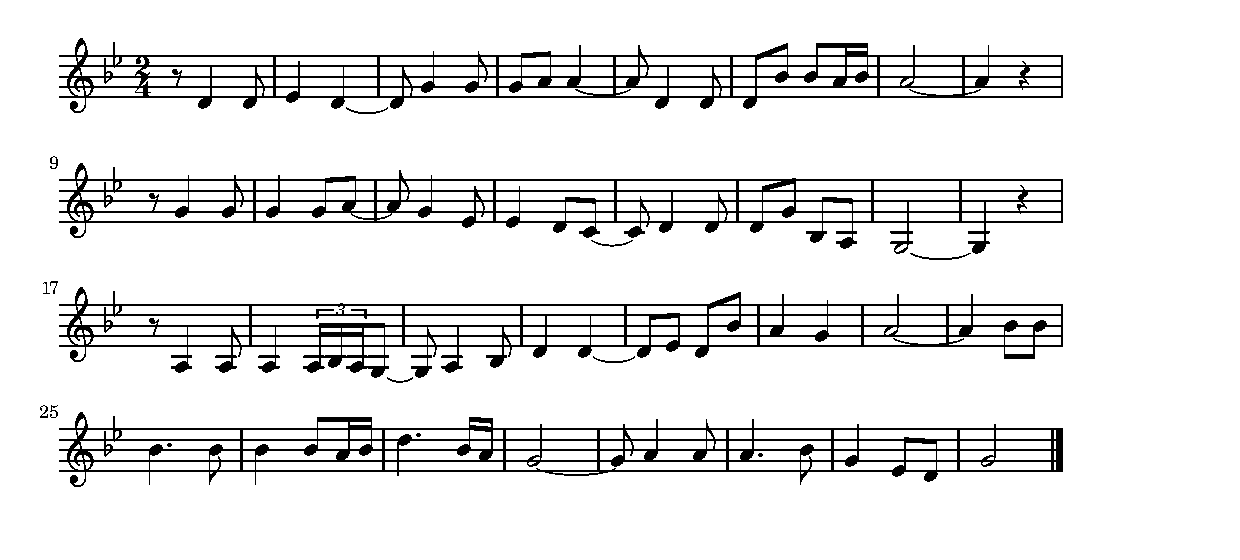
\includegraphics[clip]{wakarebune_crop.pdf}

\vspace{-10mm} \hspace{10mm}
別れ船(なごりつきないはてしない)
\index{わかれぶね@別れ船(なごりつきないはてしない)}

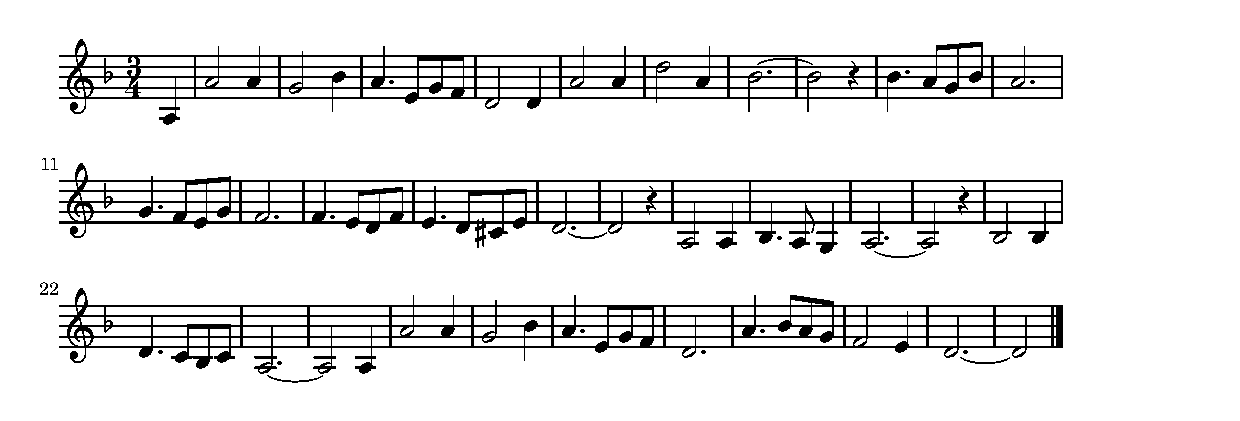
\includegraphics[clip]{mizuironowaltz_crop.pdf}

\vspace{-10mm} \hspace{10mm}
水色のワルツ(きみにあううれしさの)
\index{みずいろの@水色のワルツ(きみにあううれしさの)}

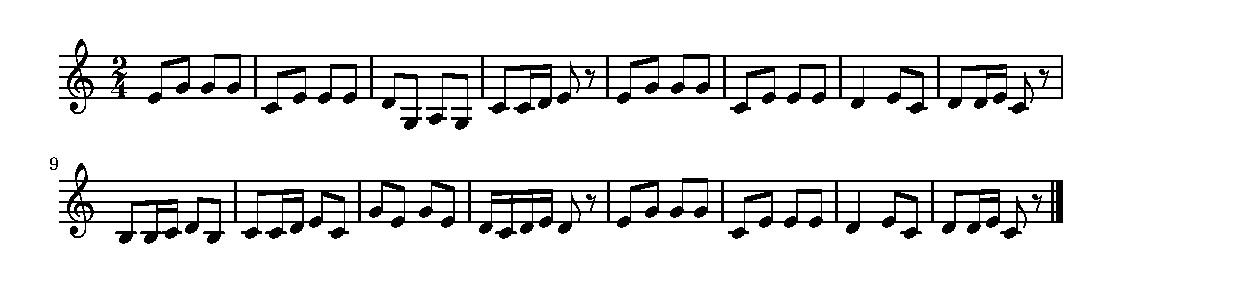
\includegraphics[clip]{muranokajiya_crop.pdf}

\vspace{-10mm} \hspace{10mm}
村の鍛冶屋(しばしもやすまずつちうつひびき)
\index{むらのかじや@村の鍛冶屋(しばしもやすまずつちうつひびき)}

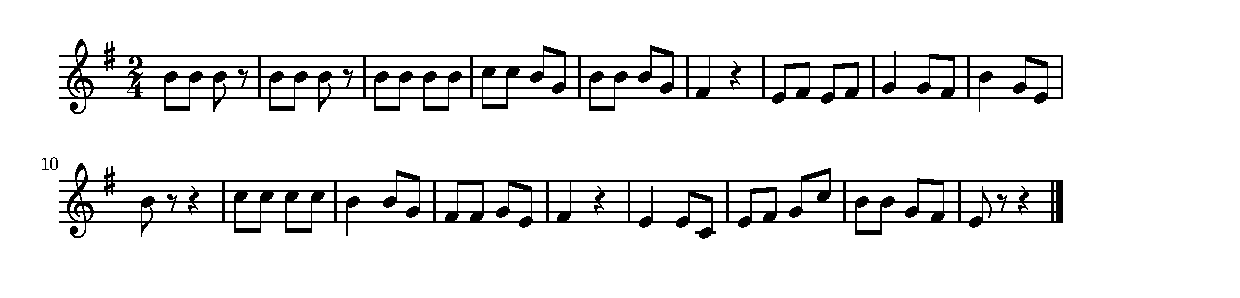
\includegraphics[clip]{naishobanashi_crop.pdf}

\vspace{-10mm} \hspace{10mm}
ないしょ話(ないしょないしょないしょのはなしはあのねのね)
\index{ないしょ@ないしょ話(ないしょないしょないしょのはなしはあのねのね)}

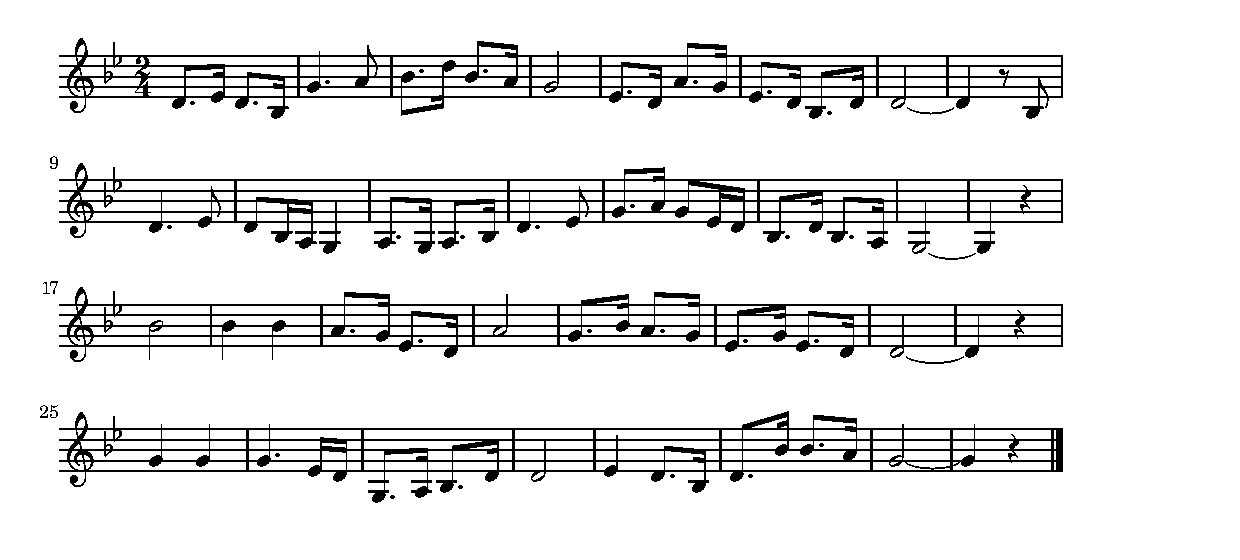
\includegraphics[clip]{nakunakobato_crop.pdf}

\vspace{-10mm} \hspace{10mm}
啼くな小鳩よ(なくなこばとよこころのつまよ)
\index{なくなこばと@啼くな小鳩よ(なくなこばとよこころのつまよ)}

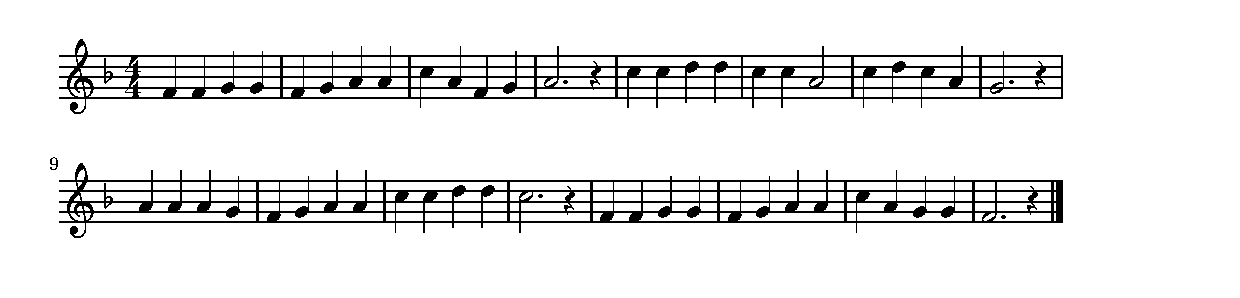
\includegraphics[clip]{ningyou_crop.pdf}

\vspace{-10mm} \hspace{10mm}
人形(わたしのにんぎょうはよいにんぎょう)
\index{にんぎょう@人形(わたしのにんぎょうはよいにんぎょう)}

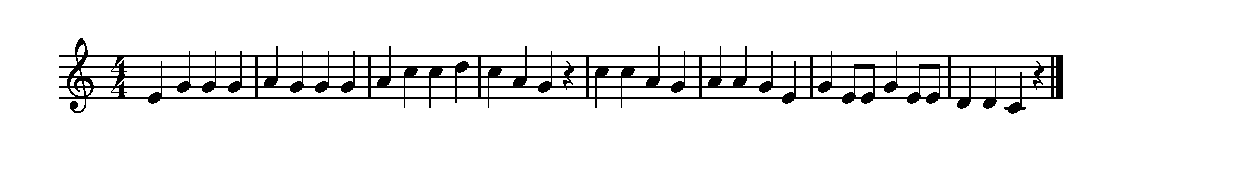
\includegraphics[clip]{ouma_crop.pdf}

\vspace{-10mm} \hspace{10mm}
おうま(おうまのおやこはなかよしこよし)
\index{おうま@おうま(おうまのおやこはなかよしこよし)}

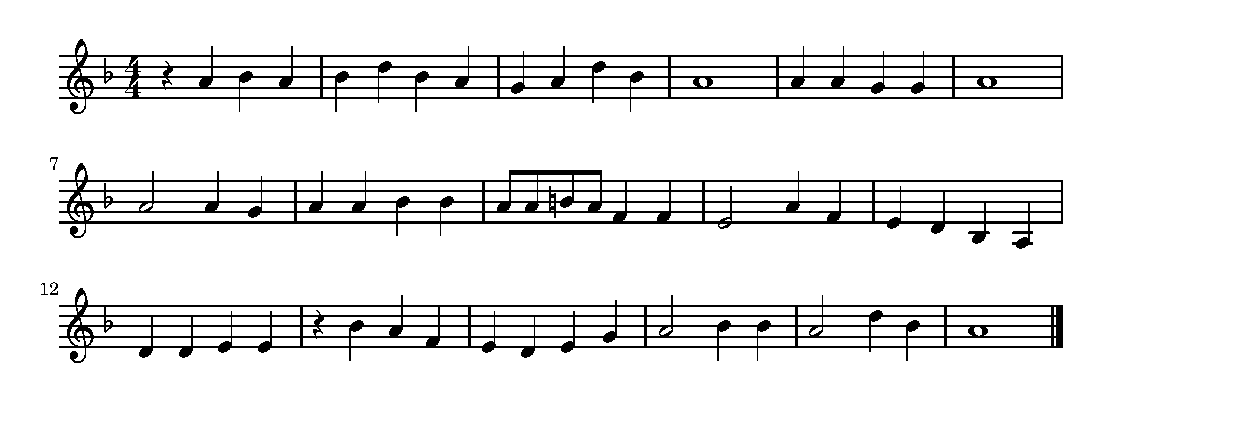
\includegraphics[clip]{oedonihonbashi_crop.pdf}

\vspace{-10mm} \hspace{10mm}
お江戸日本橋(おえどにほんばしななつだち)
\index{おえどにほんばし@お江戸日本橋(おえどにほんばしななつだち)}

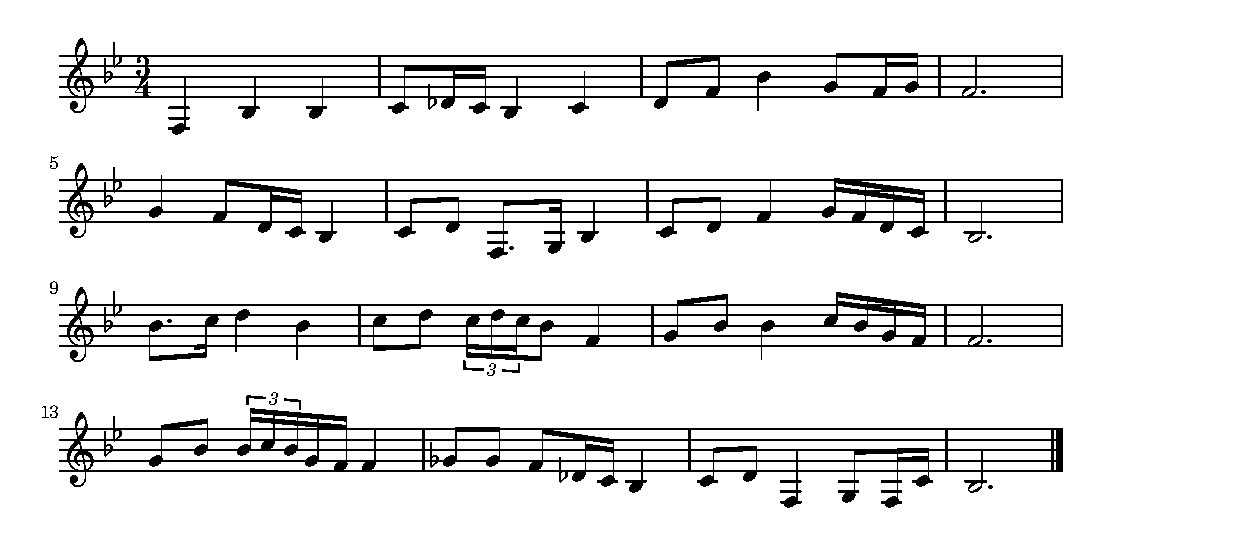
\includegraphics[clip]{otokonojunjo_crop.pdf}

\vspace{-10mm} \hspace{10mm}
男の純情(おとこいのちのじゅんじょうは)
\index{おとこの@男の純情(おとこいのちのじゅんじょうは)}

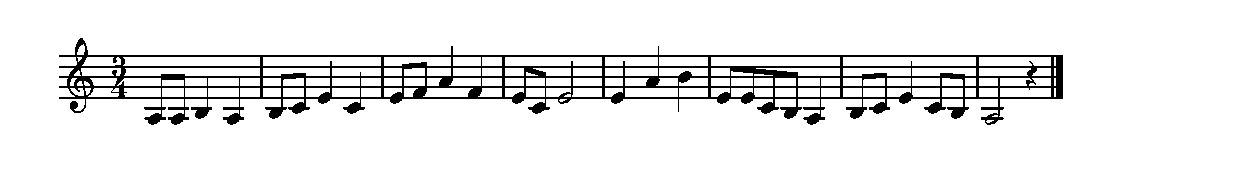
\includegraphics[clip]{kagonotori_crop.pdf}

\vspace{-10mm} \hspace{10mm}
籠の鳥(あいたさみたさにこわさをわすれ)
\index{かごのとり@籠の鳥(あいたさみたさにこわさをわすれ)}

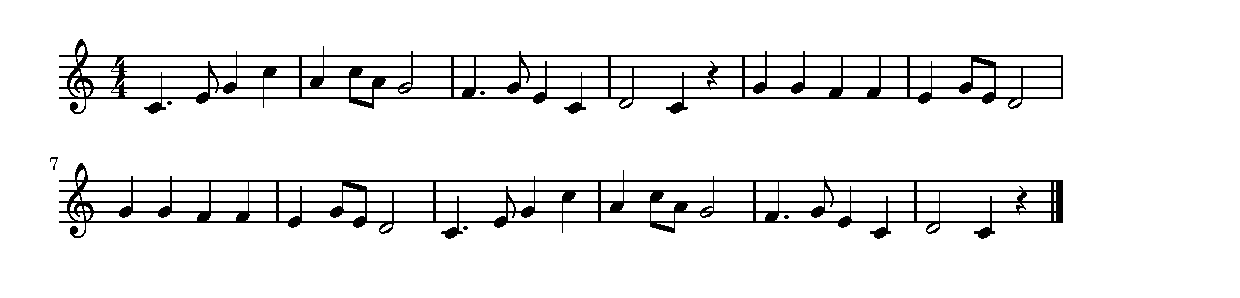
\includegraphics[clip]{kasumikakumoka_crop.pdf}

\vspace{-10mm} \hspace{10mm}
霞か雲か(かすみかくもか)
\index{かすみか@霞か雲か(かすみかくもか)}

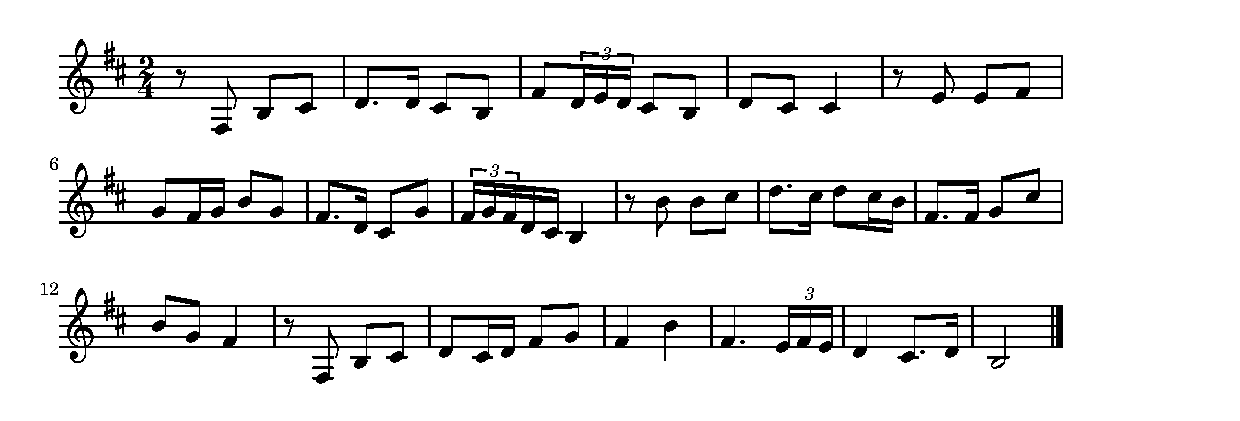
\includegraphics[clip]{aoisebirode_crop.pdf}

\vspace{-10mm} \hspace{10mm}
青い背広で(あおいせびろでこころもかるく)
\index{あおいせびろで@青い背広で(あおいせびろでこころもかるく)}

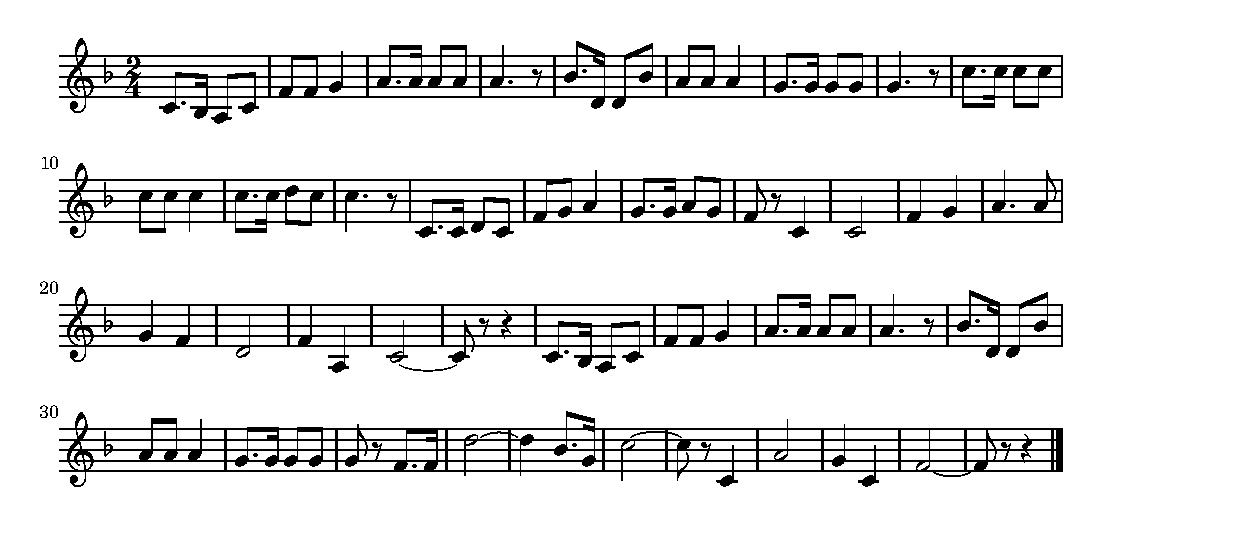
\includegraphics[clip]{aikokukoushinkyoku_crop.pdf}

\vspace{-10mm} \hspace{10mm}
愛国行進曲(みよとうかいのそらあけて)
\index{あいこく@愛国行進曲(みよとうかいのそらあけて)}

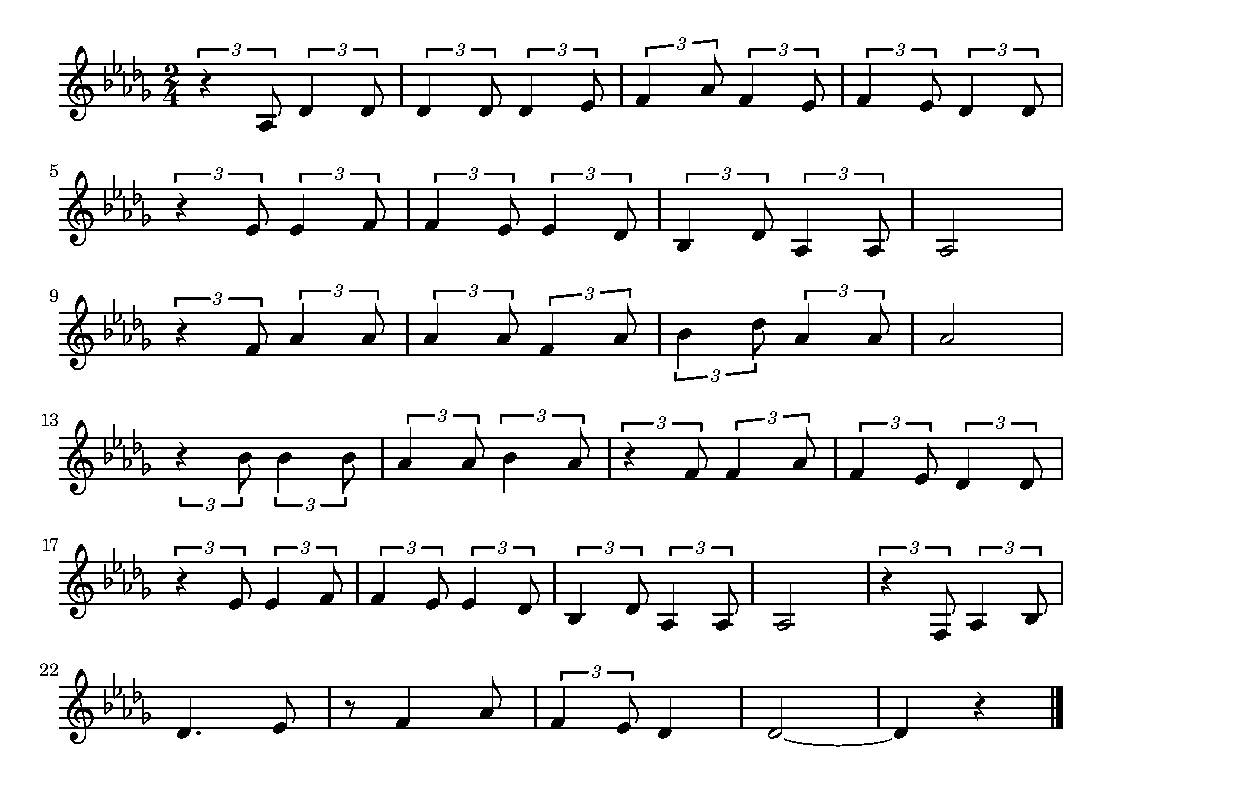
\includegraphics[clip]{otomisan_crop.pdf}

\vspace{-10mm} \hspace{10mm}
お富さん(いきなくろべいみこしのまつに)
\index{おとみさん@お富さん(いきなくろべいみこしのまつに)}

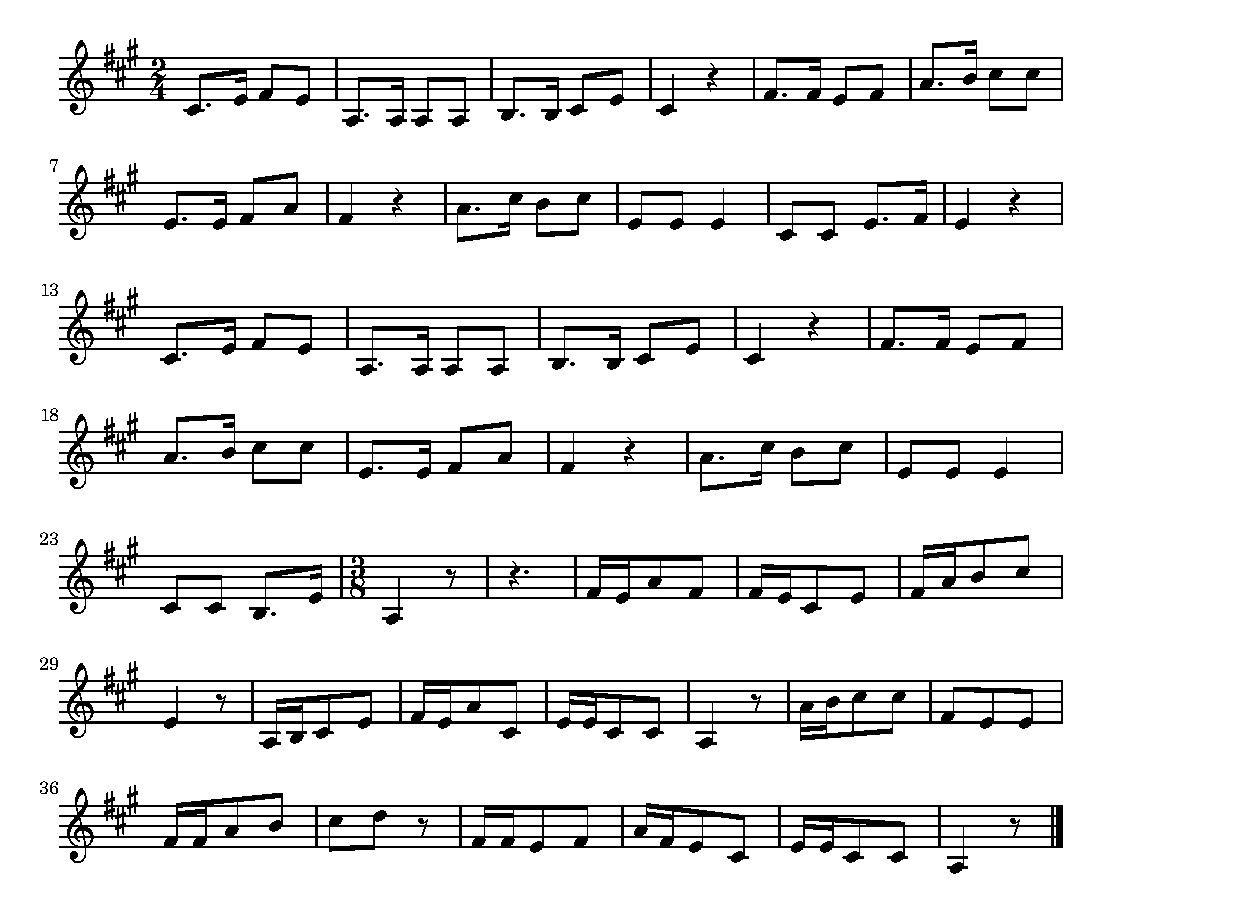
\includegraphics[clip]{canary_crop.pdf}

\vspace{-10mm} \hspace{10mm}
かなりや(うたをわすれたかなりやは)
\index{かなりや@かなりや(うたをわすれたかなりやは)}

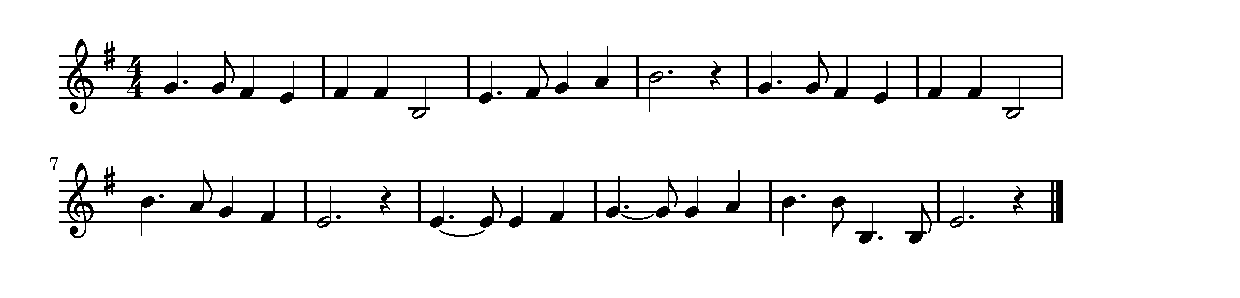
\includegraphics[clip]{kamakura_crop.pdf}

\vspace{-10mm} \hspace{10mm}
鎌倉(しちりがはまのいそづたい)
\index{かまくら@鎌倉(しちりがはまのいそづたい)}

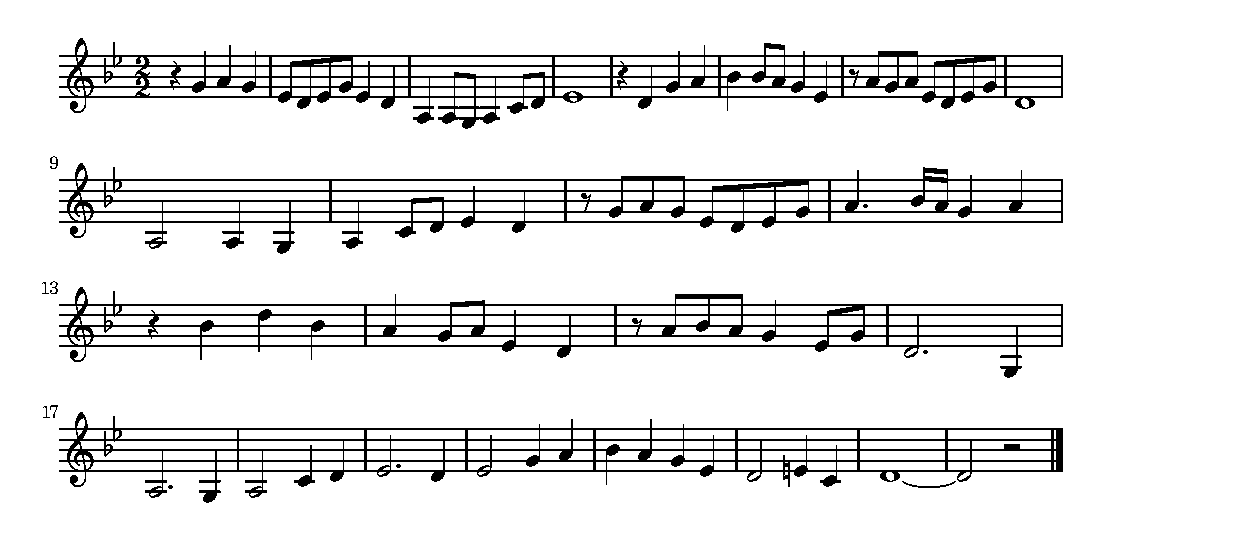
\includegraphics[clip]{gionkouta_crop.pdf}

\vspace{-10mm} \hspace{10mm}
祇園小唄(つきはおぼろにひがしやま)
\index{ぎおんこうた@祇園小唄(つきはおぼろにひがしやま)}

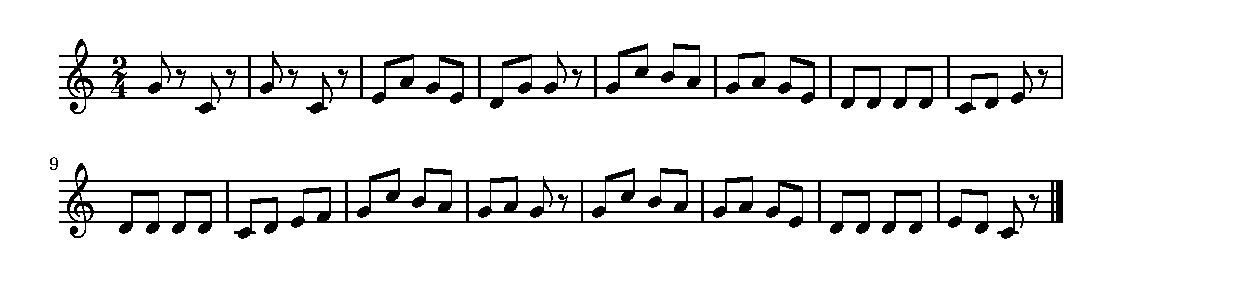
\includegraphics[clip]{kouma_crop.pdf}

\vspace{-10mm} \hspace{10mm}
こうま(はいしいはいしいあゆめよこうま)
\index{こうま@こうま(はいしいはいしいあゆめよこうま)}

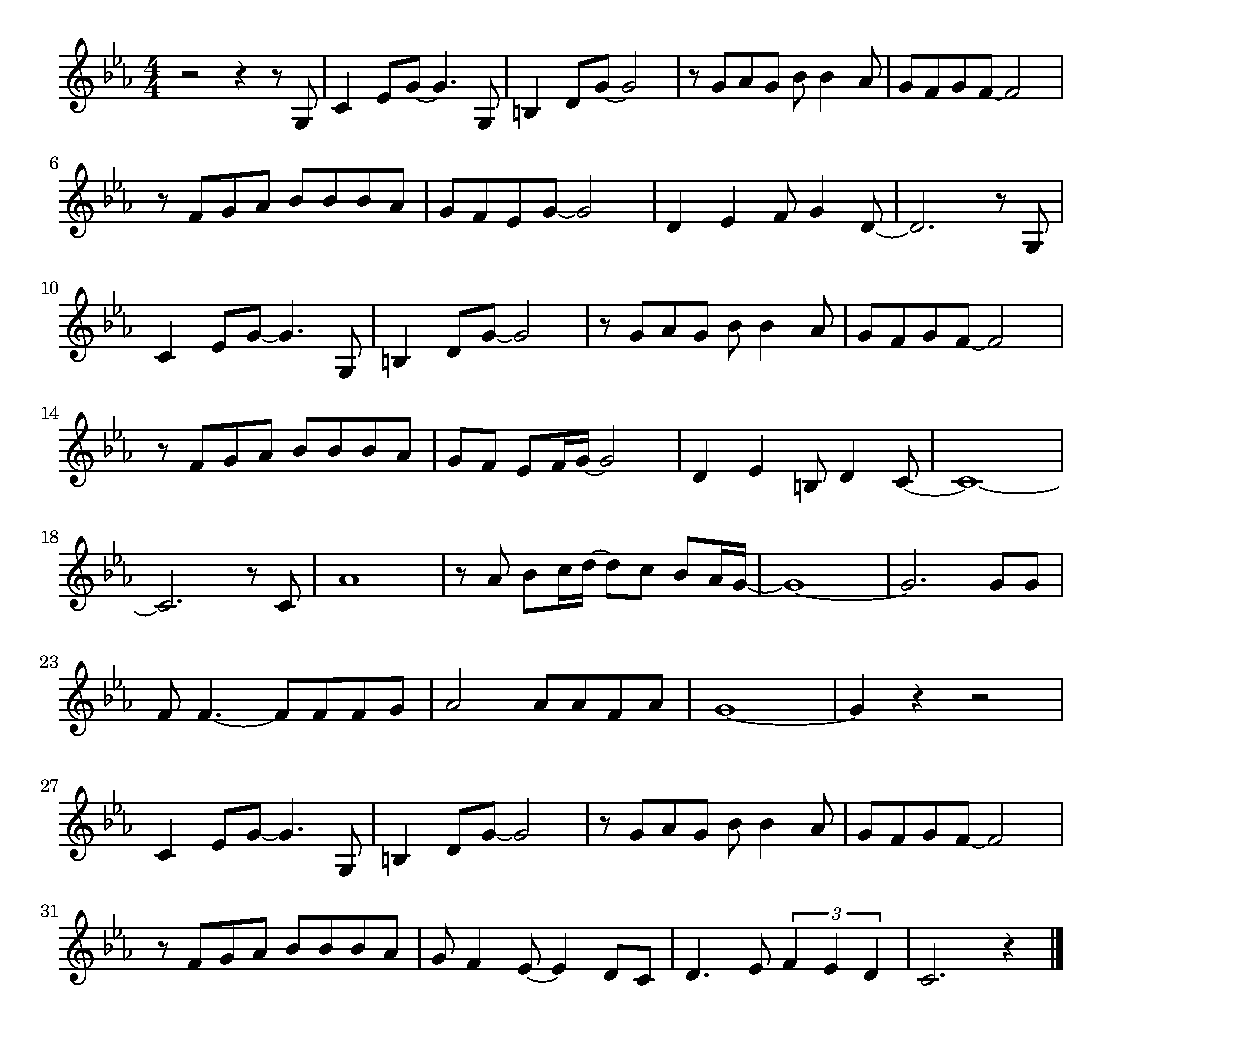
\includegraphics[clip]{iihitabidachi_crop.pdf}

\vspace{-10mm} \hspace{10mm}
いい日旅立ち(ゆきどけまじかの)
\index{いいひ@いい日旅立ち(ゆきどけまじかの)}

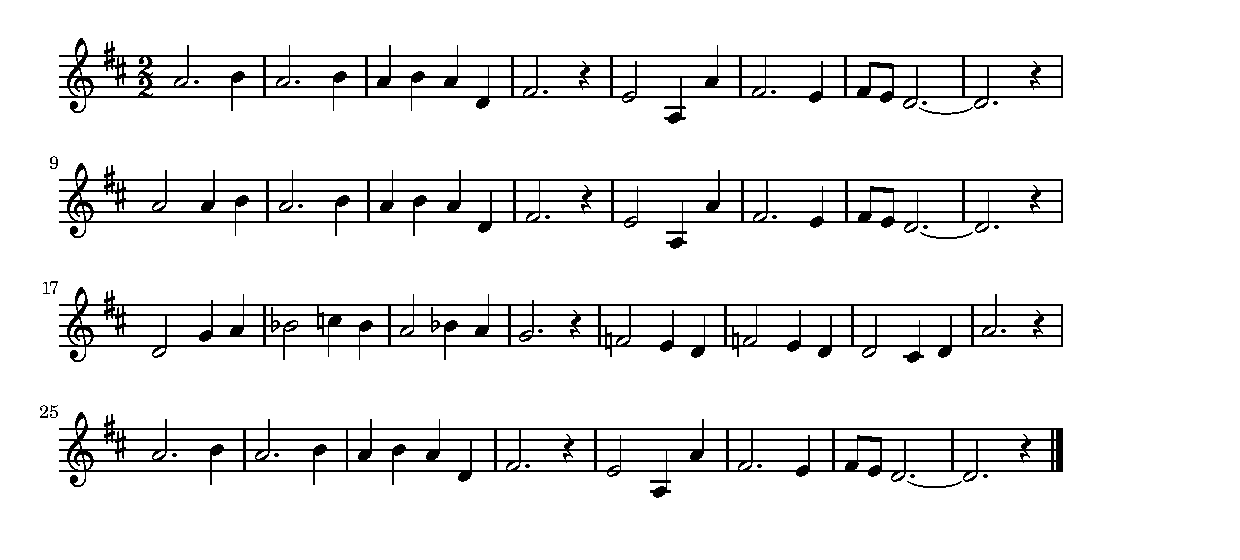
\includegraphics[clip]{arabianouta_crop.pdf}

\vspace{-10mm} \hspace{10mm}
アラビアの唄(さばくにひがおちて)
\index{あらびあ@アラビアの唄(さばくにひがおちて)}

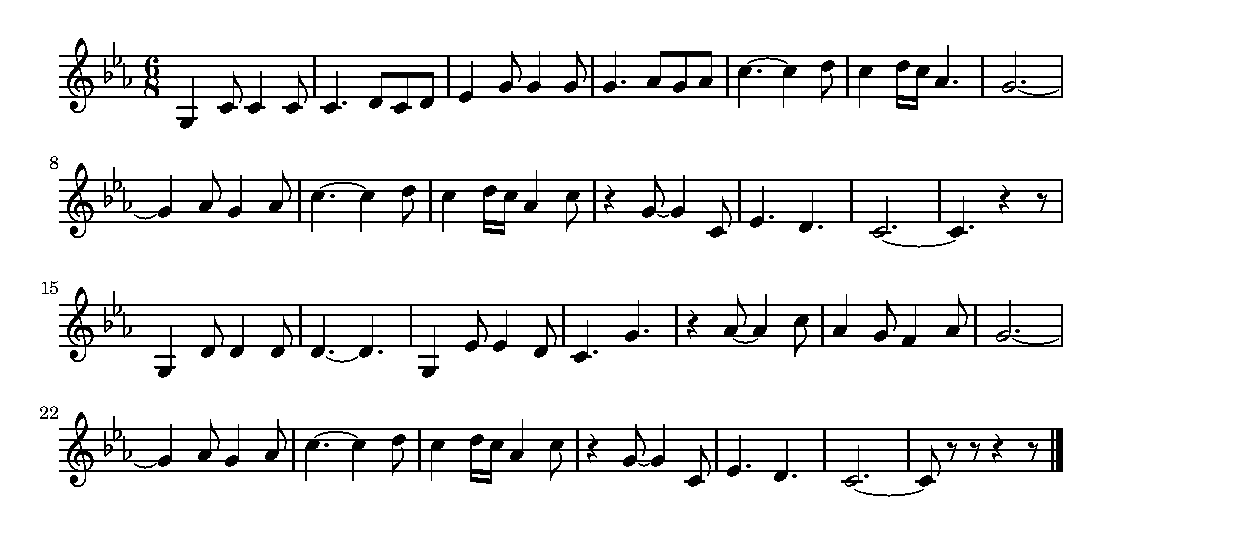
\includegraphics[clip]{khabarovsk_crop.pdf}

\vspace{-10mm} \hspace{10mm}
ハバロフスク小唄
\index{はばろふすく@ハバロフスク小唄}

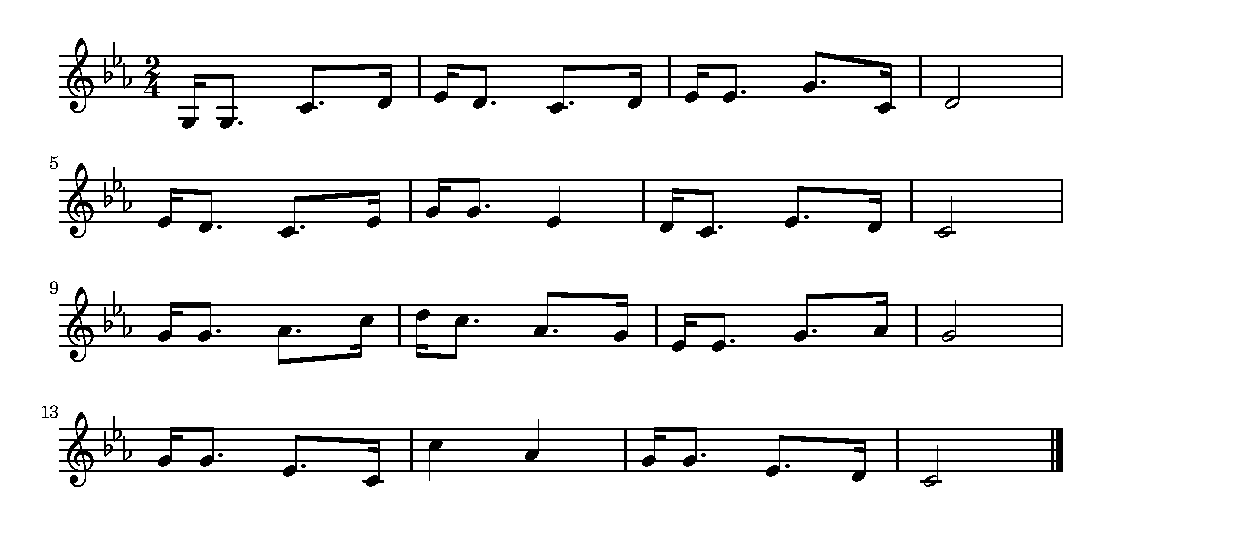
\includegraphics[clip]{hitowokouruuta_crop.pdf}

\vspace{-10mm} \hspace{10mm}
人を恋うる歌(つまをめとらばさいたけて)
\index{ひとをこうる@人を恋うる歌(つまをめとらばさいたけて)}

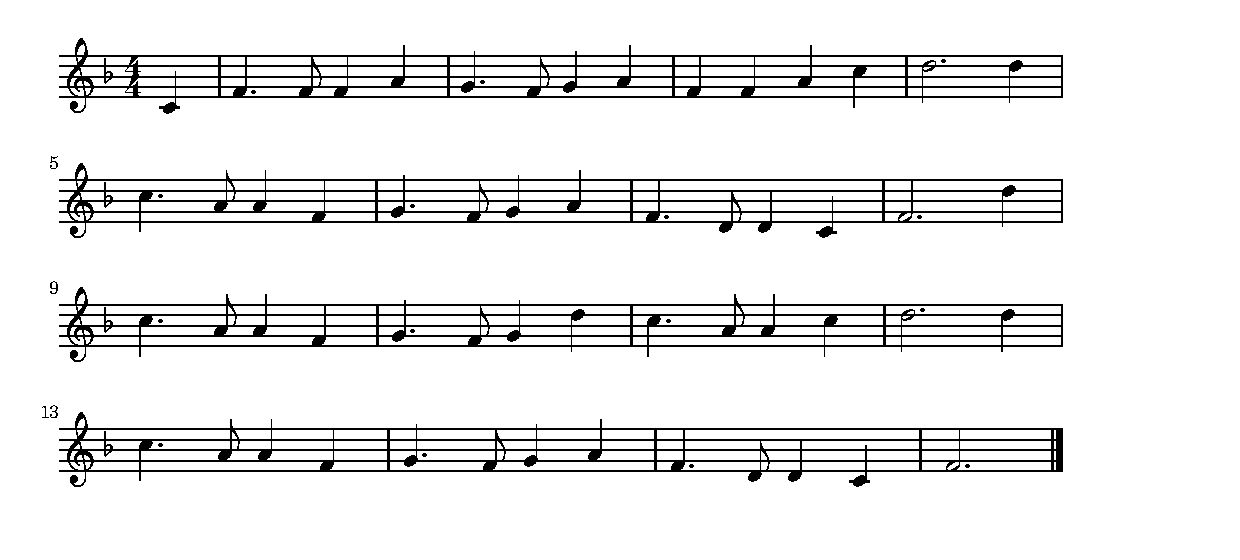
\includegraphics[clip]{hotarunohikari_crop.pdf}

\vspace{-10mm} \hspace{10mm}
蛍の光(ほたるのひかりまどのゆき)
\index{ほたるのひかり@蛍の光(ほたるのひかりまどのゆき)}

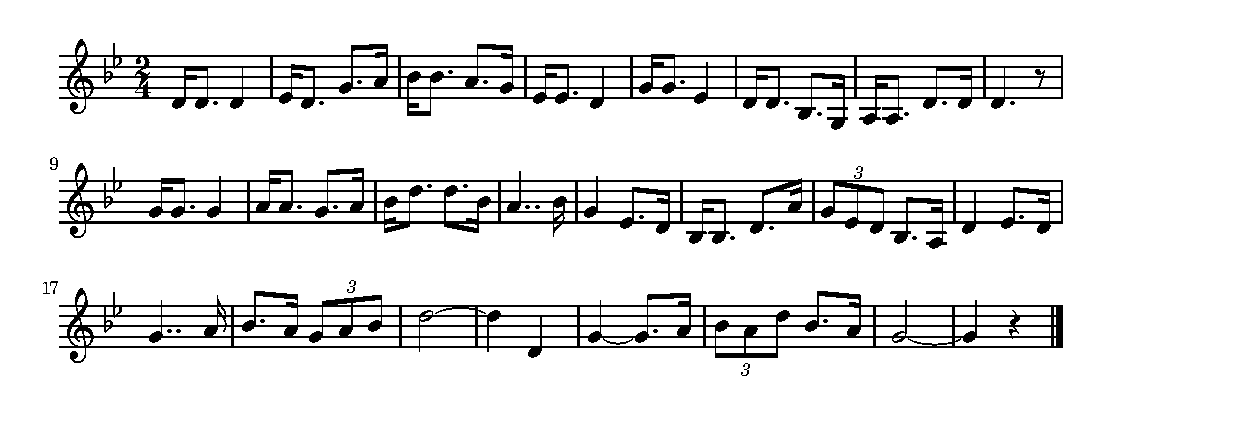
\includegraphics[clip]{mugitoheitai_crop.pdf}

\vspace{-10mm} \hspace{10mm}
麦と兵隊(じょしゅうじょしゅうとじんばはすすむ)
\index{むぎと@麦と兵隊(じょしゅうじょしゅうとじんばはすすむ)}

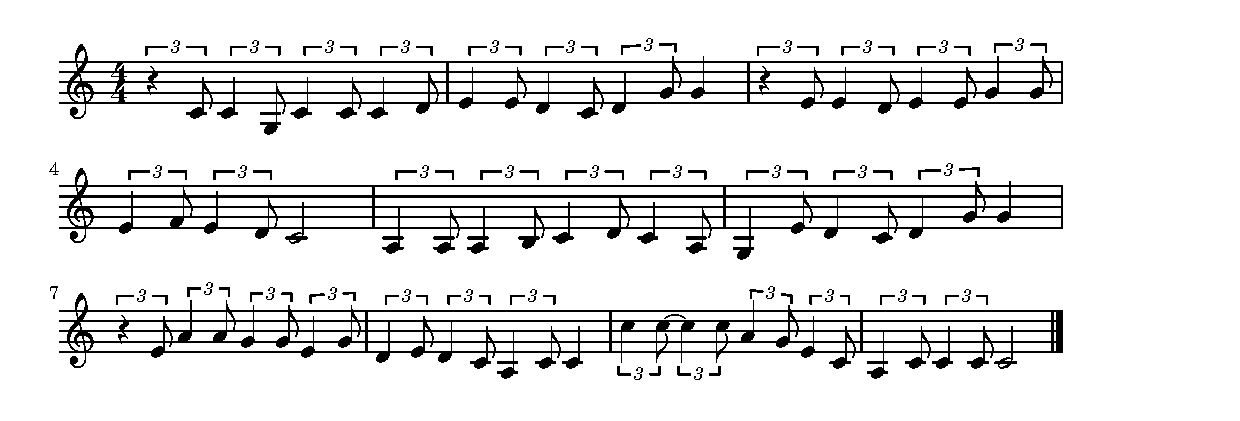
\includegraphics[clip]{sudarabushi_crop.pdf}

\vspace{-10mm} \hspace{10mm}
スーダラ節(植木等、ちょいといっぱいのつもりでのんで)
\index{すーだら@スーダラ節(植木等、ちょいといっぱいのつもりでのんで)}

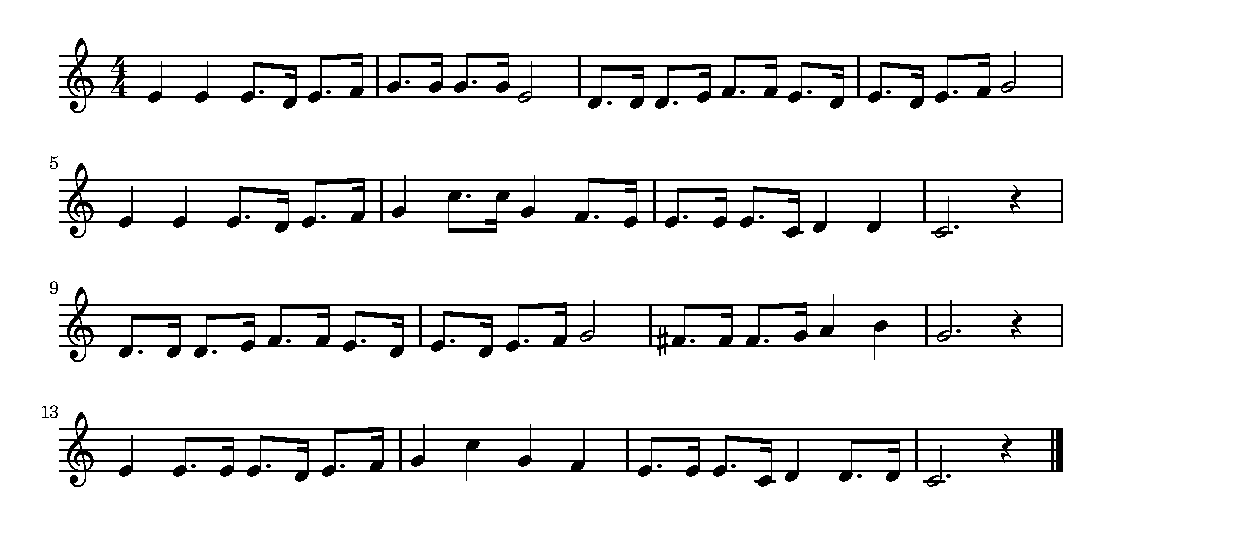
\includegraphics[clip]{tabakoya_crop.pdf}

\vspace{-10mm} \hspace{10mm}
たばこやの娘(むこうよこちょうのたばこやの)
\index{たばこ@たばこやの娘(むこうよこちょうのたばこやの)}


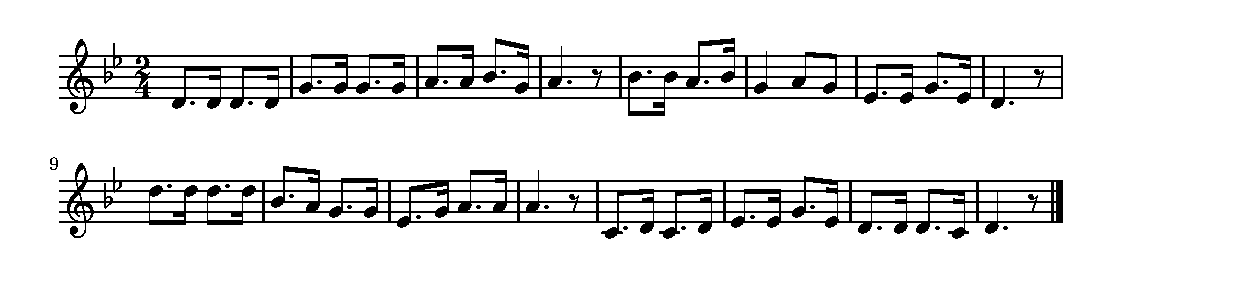
\includegraphics[clip]{senyu_crop.pdf}

\vspace{-10mm} \hspace{10mm}
戦友(ここはおくにをなんびゃくり)
\index{せんゆう@戦友(ここはおくにをなんびゃくり)}

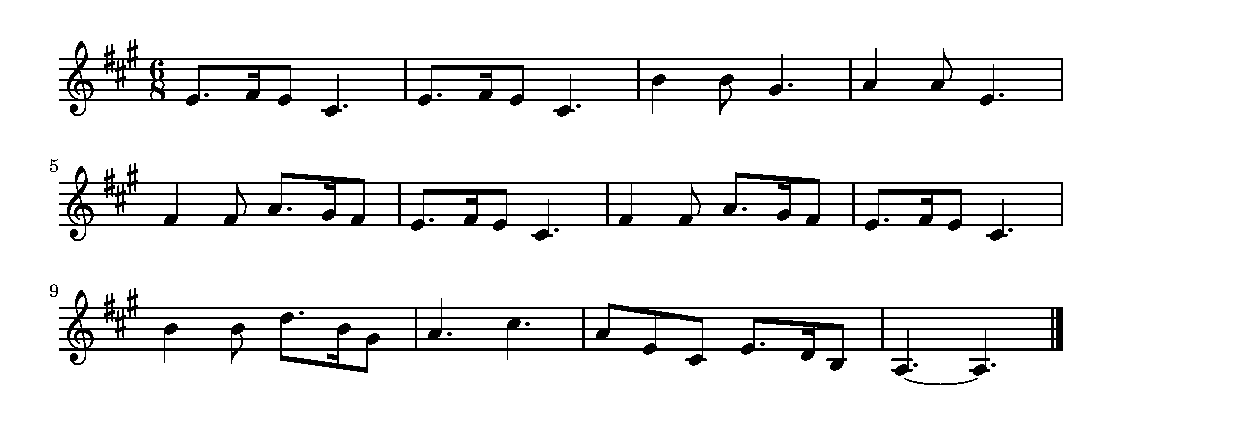
\includegraphics[clip]{kiyoshi_crop.pdf}

\vspace{-10mm} \hspace{10mm}
聖夜(きよしこのよる)
\index{きよしこのよる@聖夜(きよしこのよる)}

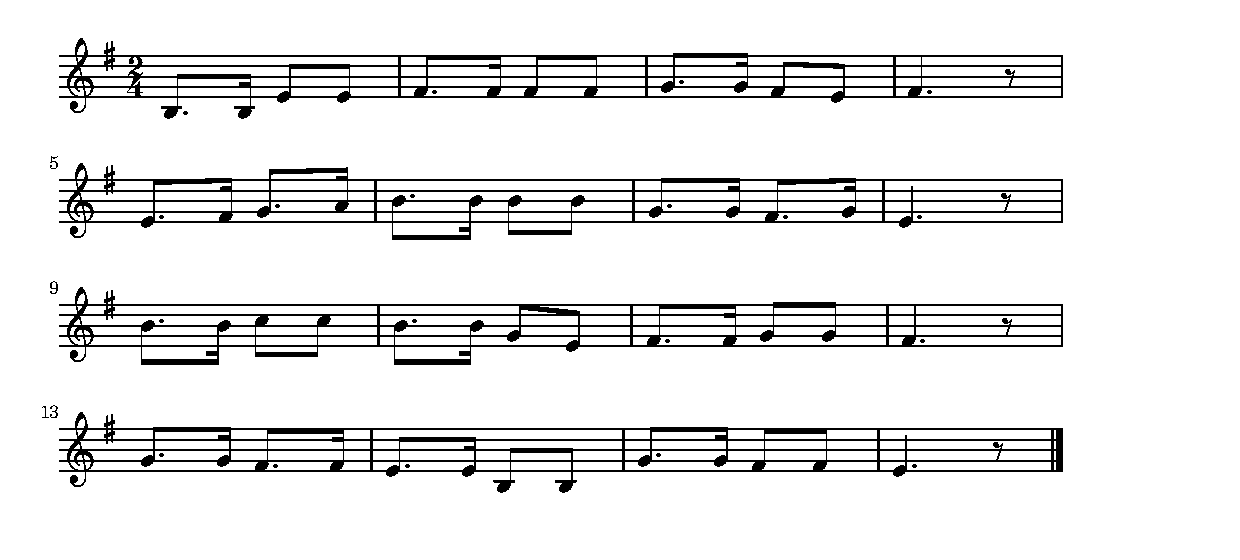
\includegraphics[clip]{suishiei_crop.pdf}

\vspace{-10mm} \hspace{10mm}
水師営の会見(りょじゅんかいじょうやくなりて)
\index{すいしえい@水師営の会見(りょじゅんかいじょうやくなりて)}

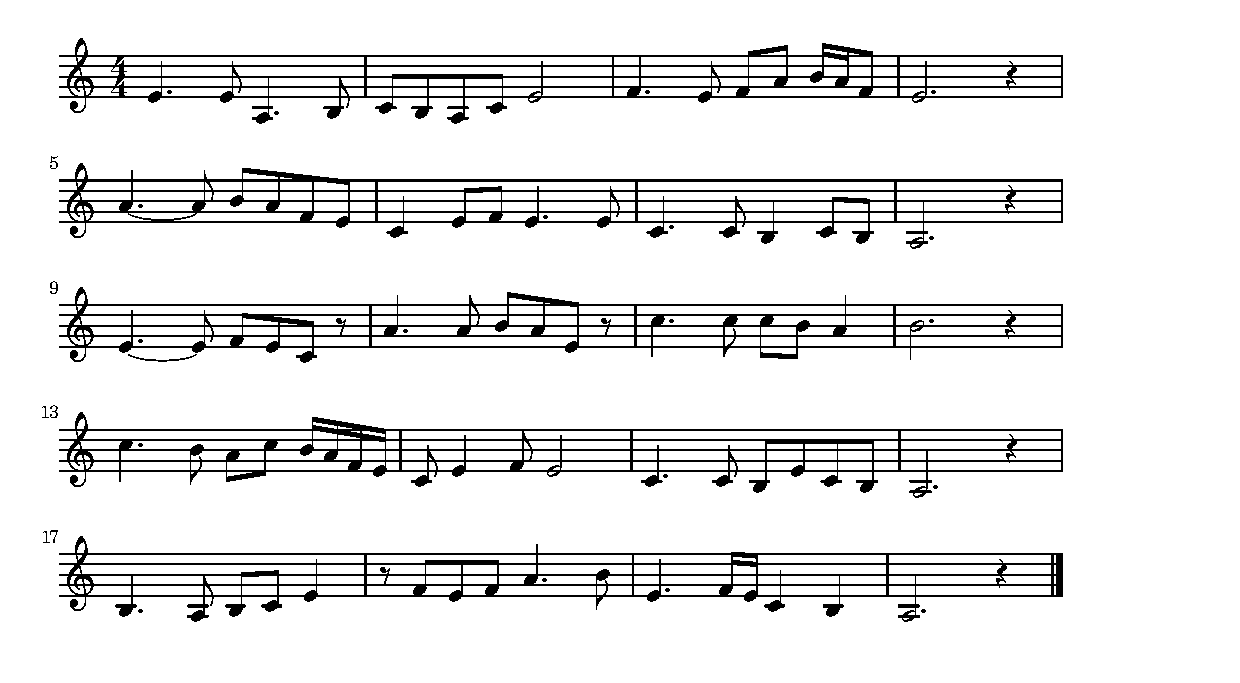
\includegraphics[clip]{muntinlupa_crop.pdf}

\vspace{-10mm} \hspace{10mm}
ああモンテンルパの夜は更けて(モンテンルパの夜は更けて。Muntinlupa, フィリピン)
\index{ああもんてんるぱ@ああモンテンルパの夜は更けて(Muntinlupa, フィリピン)}

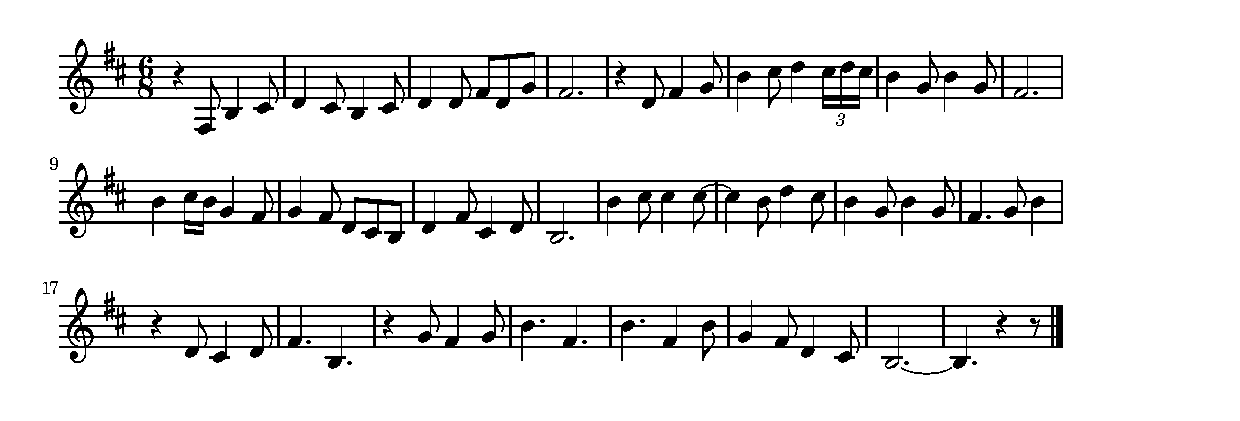
\includegraphics[clip]{aasorenanoni_crop.pdf}

\vspace{-10mm} \hspace{10mm}
ああそれなのに(そらにゃきょうもあどばるん)
\index{ああそれ@ああそれなのに(そらにゃきょうもあどばるん)}

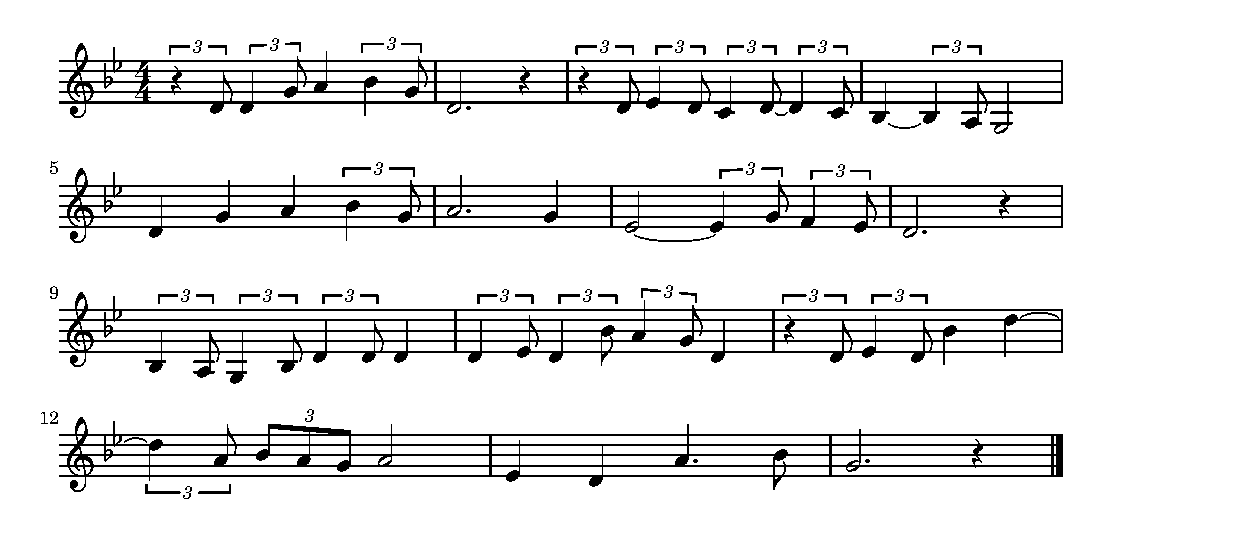
\includegraphics[clip]{kiminonawa_crop.pdf}

\vspace{-10mm} \hspace{10mm}
君の名は(きみのなはとたずねしひとあり)
\index{きみのなは@君の名は(きみのなはとたずねしひとあり)}

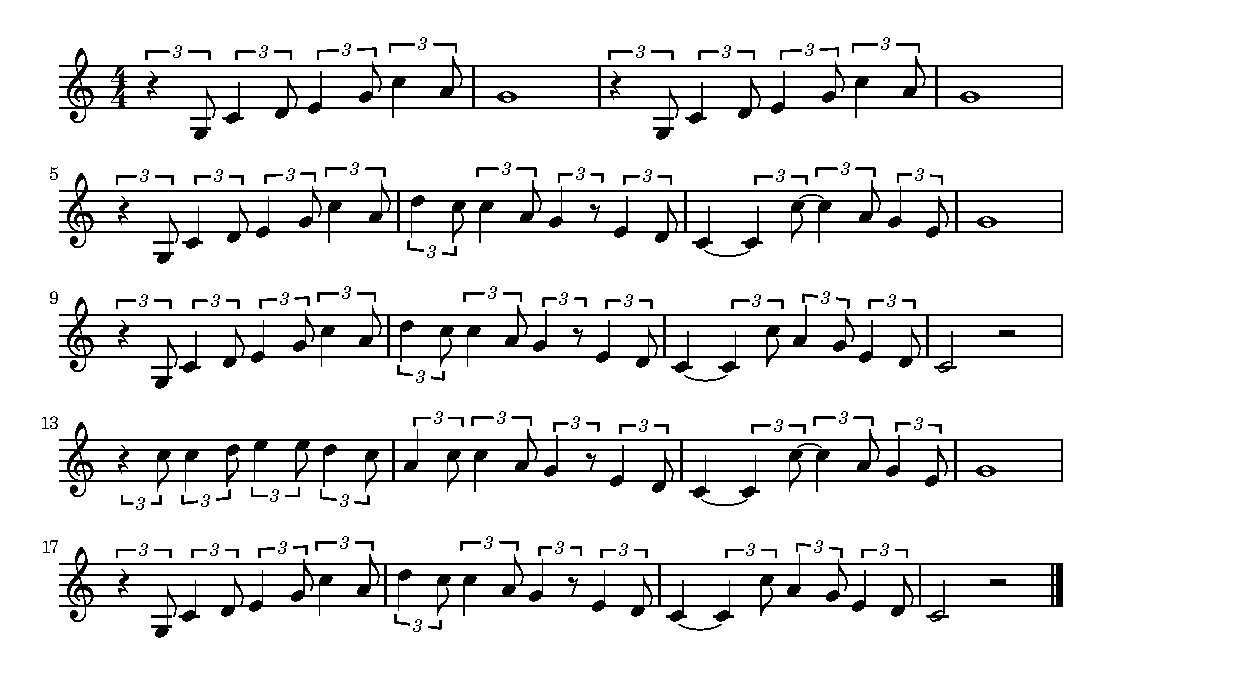
\includegraphics[clip]{kirameku_crop.pdf}

\vspace{-10mm} \hspace{10mm}
燦めく星座(おとこじゅんじょうのあいのほしのいろ)
\index{きらめく@燦めく星座(おとこじゅんじょうのあいのほしのいろ)}

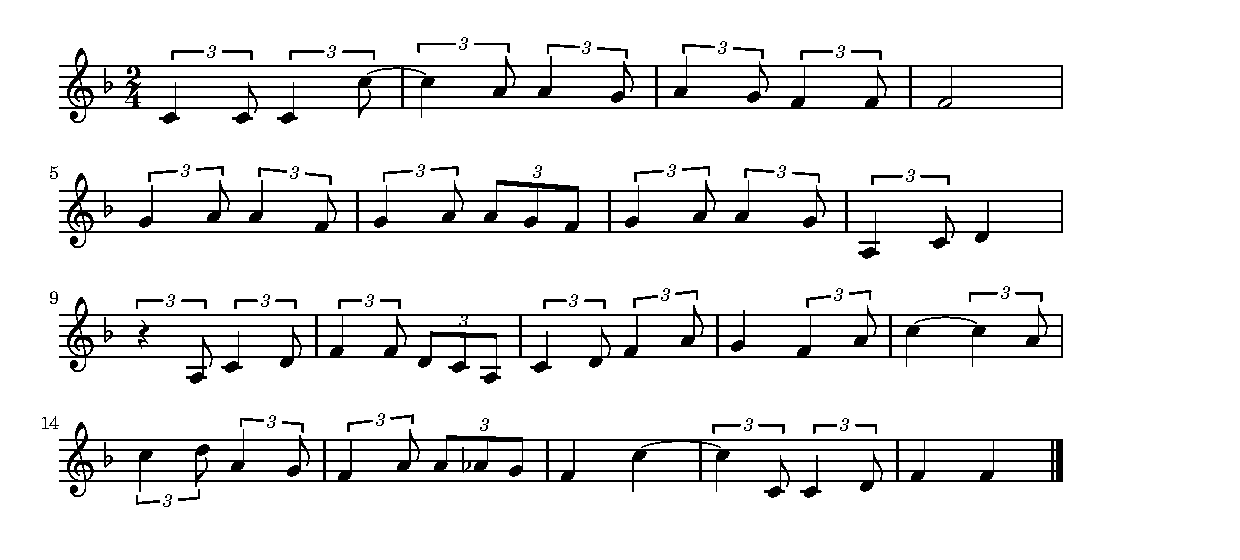
\includegraphics[clip]{tonkobushi_crop.pdf}

\vspace{-10mm} \hspace{10mm}
トンコ節(あなたのくれたおびどめの)
\index{とんこ@トンコ節(あなたのくれたおびどめの)}

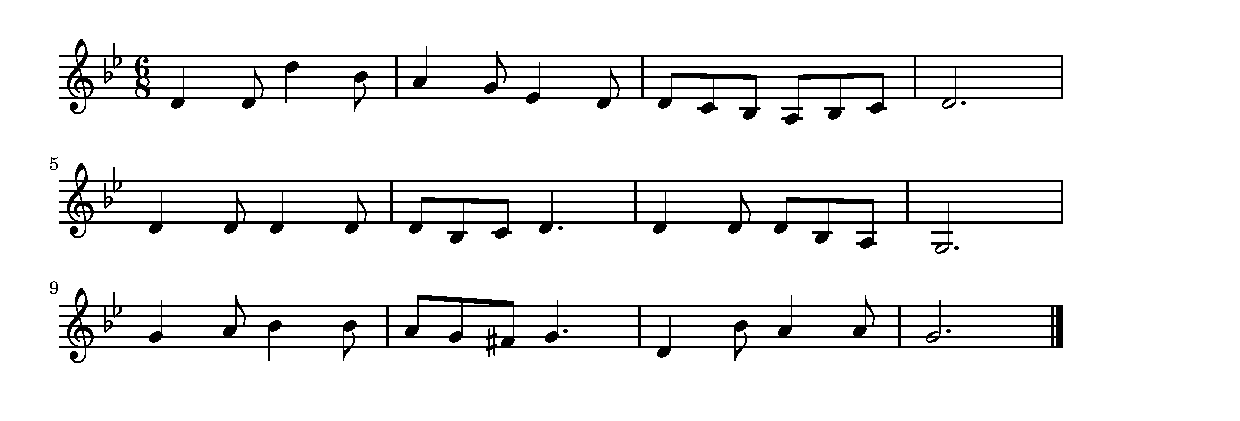
\includegraphics[clip]{yoimachigusa_crop.pdf}

\vspace{-10mm} \hspace{10mm}
宵待草(まてどくらせどこぬひとを)
\index{よいまちぐさ@宵待草(まてどくらせどこぬひとを)}

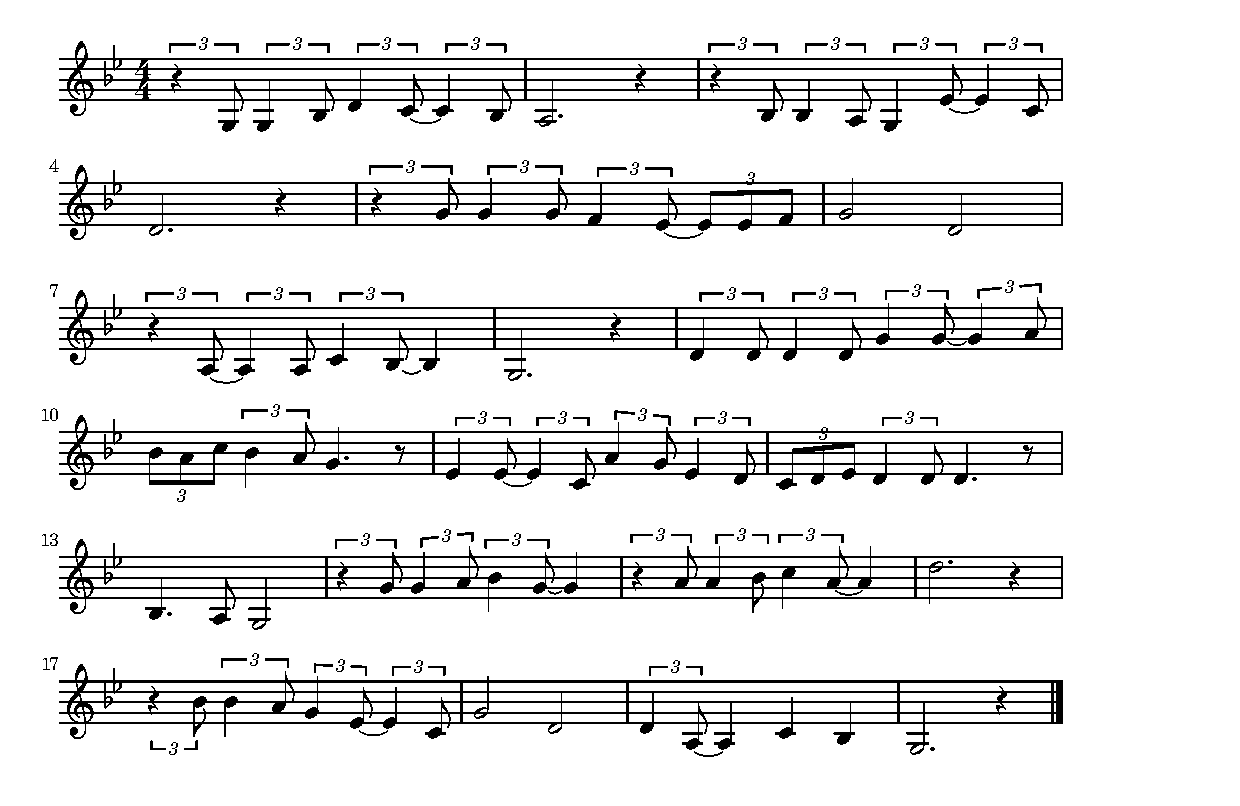
\includegraphics[clip]{natsukashinoblues_crop.pdf}

\vspace{-10mm} \hspace{10mm}
懐かしのブルース(ふるいにっきのぺーじには)
\index{なつかしの@懐かしのブルース(ふるいにっきのぺーじには)}

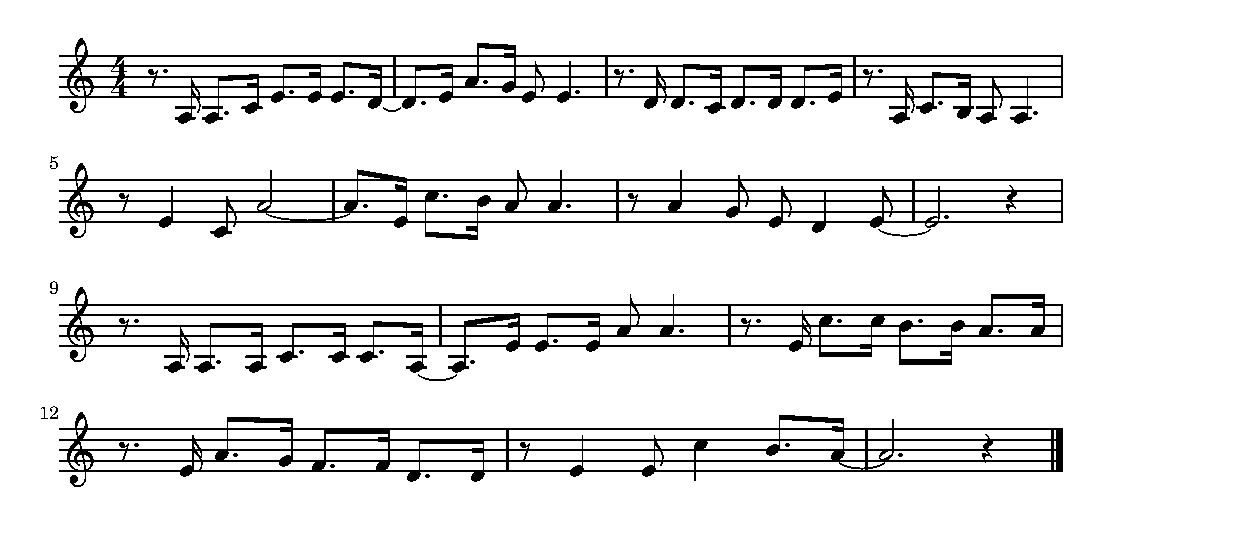
\includegraphics[clip]{kanashikikuchibue_crop.pdf}

\vspace{-10mm} \hspace{10mm}
悲しき口笛(おかのほてるのあかいひも)
\index{かなしき@悲しき口笛(おかのほてるのあかいひも)}


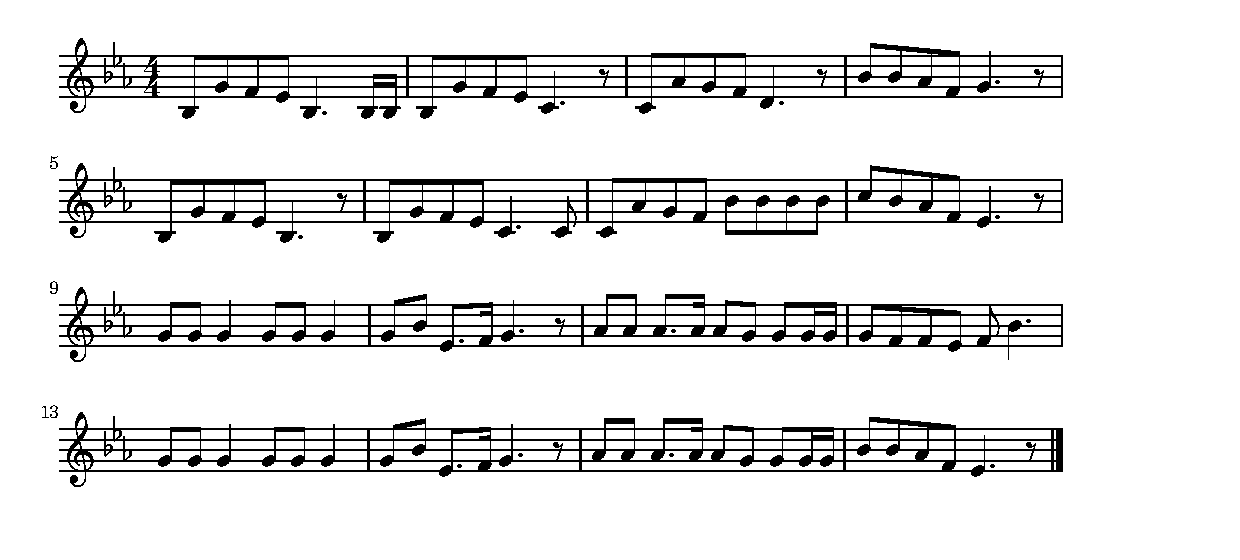
\includegraphics[clip]{jinglebell_crop.pdf}

\vspace{-10mm} \hspace{10mm}
ジングル・ベル(クリスマス。のをこえておかをこえ)
\index{じんぐる@ジングル・ベル(クリスマス。のをこえておかをこえ)}
\index{くりすます@ジングル・ベル(クリスマス。のをこえておかをこえ)}

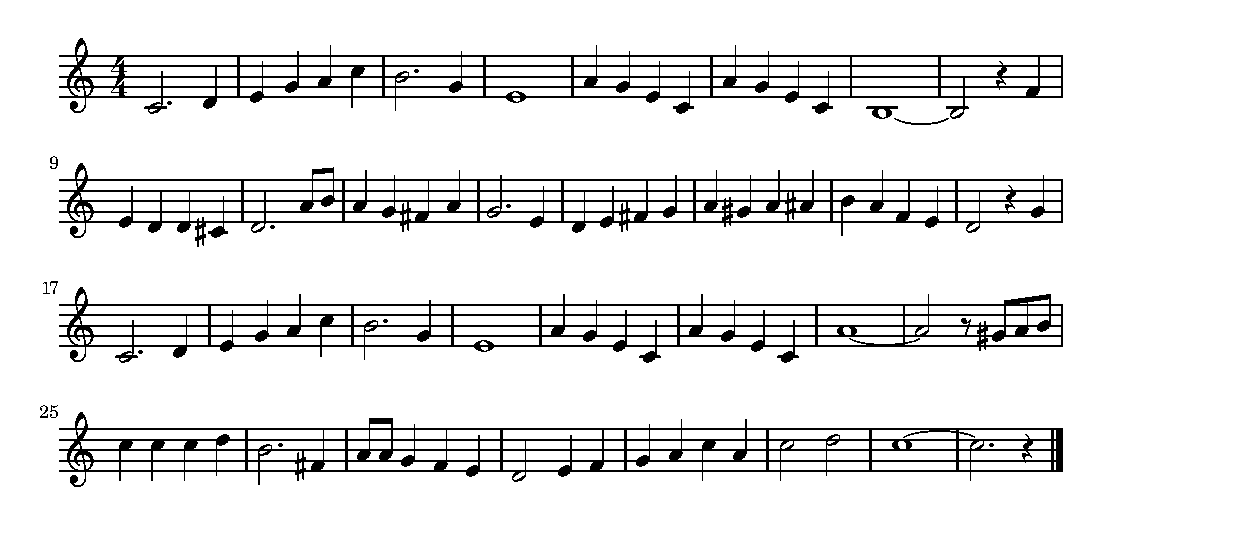
\includegraphics[clip]{mommykisssanta_crop.pdf}

\vspace{-10mm} \hspace{10mm}
ママがサンタにキスをした(クリスマス。I Saw Mommy Kissing Santa Claus)
\index{ままが@ママがサンタにキスをした(クリスマス。I Saw Mommy Kissing Santa Claus)}
\index{くりすます@ママがサンタにキスをした(クリスマス。I Saw Mommy Kissing Santa Claus)}

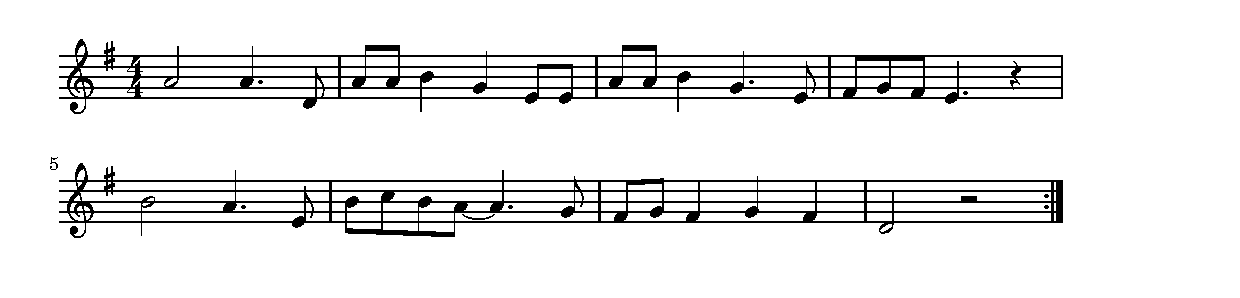
\includegraphics[clip]{lastchristmas_crop.pdf}

\vspace{-10mm} \hspace{10mm}
ラスト・クリスマス(ワム!)
\index{らすと@ラスト・クリスマス(ワム!)}
\index{くりすます@ラスト・クリスマス(ワム!)}

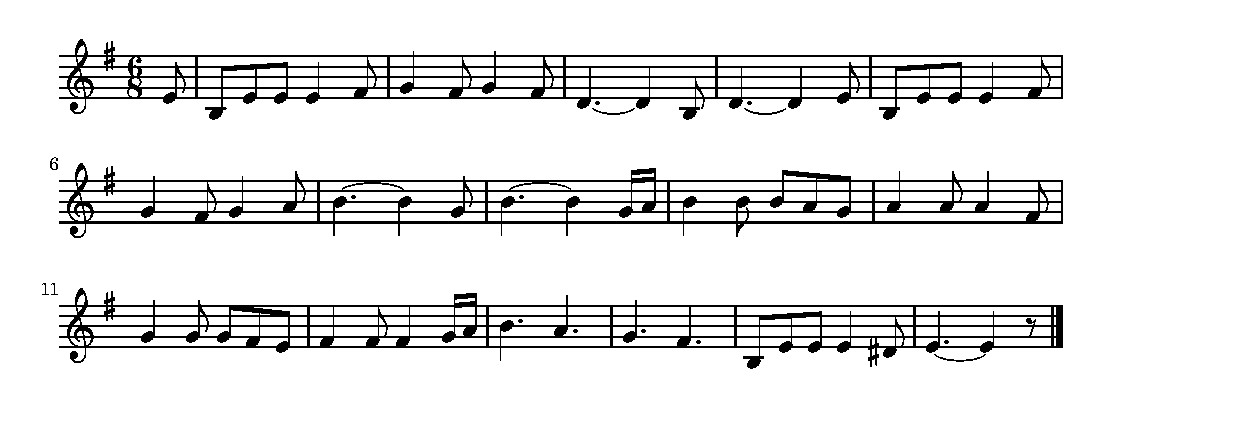
\includegraphics[clip]{whenjohnny_crop.pdf}

\vspace{-10mm} \hspace{10mm}
ジョニーが凱旋するとき(When Johnny Comes Marching Home)
\index{じょーにー@ジョニーが凱旋するとき(When Johnny Comes Marching Home)}

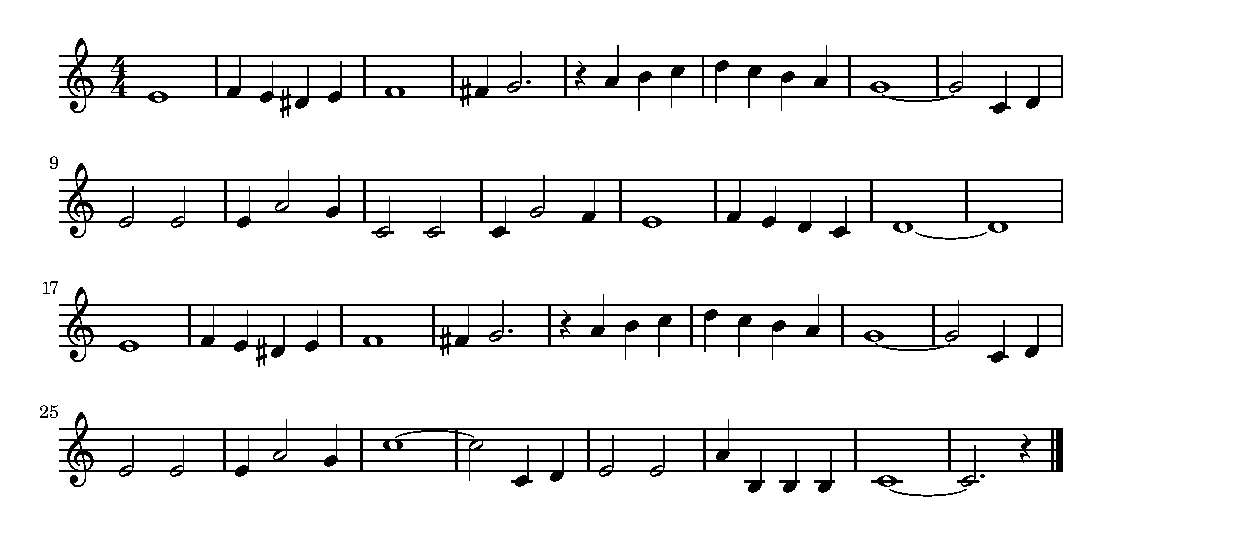
\includegraphics[clip]{whitechristmas_crop.pdf}

\vspace{-10mm} \hspace{10mm}
ホワイト・クリスマス
\index{ほわいと@ホワイト・クリスマス}
\index{くりすます@ホワイト・クリスマス}

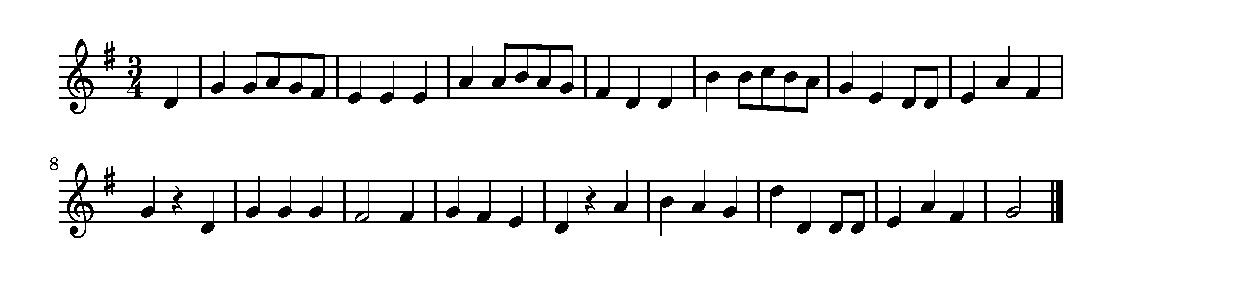
\includegraphics[clip]{omedetouchristmas_crop.pdf}

\vspace{-10mm} \hspace{10mm}
おめでとうクリスマス(We Wish You a Merry Christmas)
\index{おめでとう@おめでとうクリスマス(We Wish You a Merry Christmas)}
\index{くりすます@おめでとうクリスマス(We Wish You a Merry Christmas)}

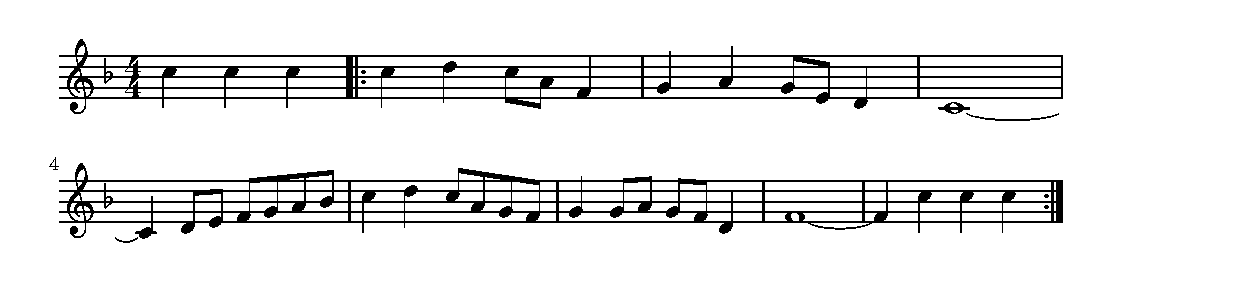
\includegraphics[clip]{sorisuberi_crop.pdf}

\vspace{-10mm} \hspace{10mm}
そりすべり(リロイ・アンダーソン。クリスマス)
\index{そりすべり@そりすべり(リロイ・アンダーソン。クリスマス)}
\index{くりすます@そりすべり(リロイ・アンダーソン。クリスマス)}

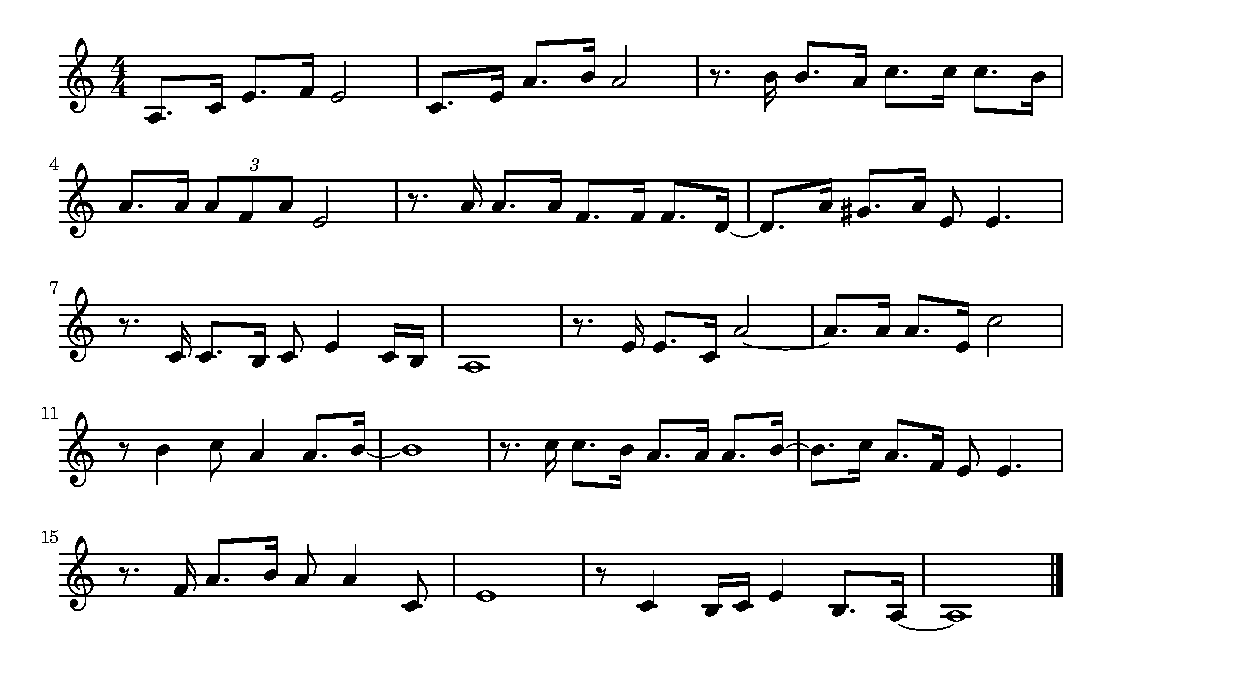
\includegraphics[clip]{sukidatta_crop.pdf}

\vspace{-10mm} \hspace{10mm}
好きだった(すきだったうそじゃなかったすきだった)
\index{すきだった@好きだった(すきだったうそじゃなかったすきだった)}

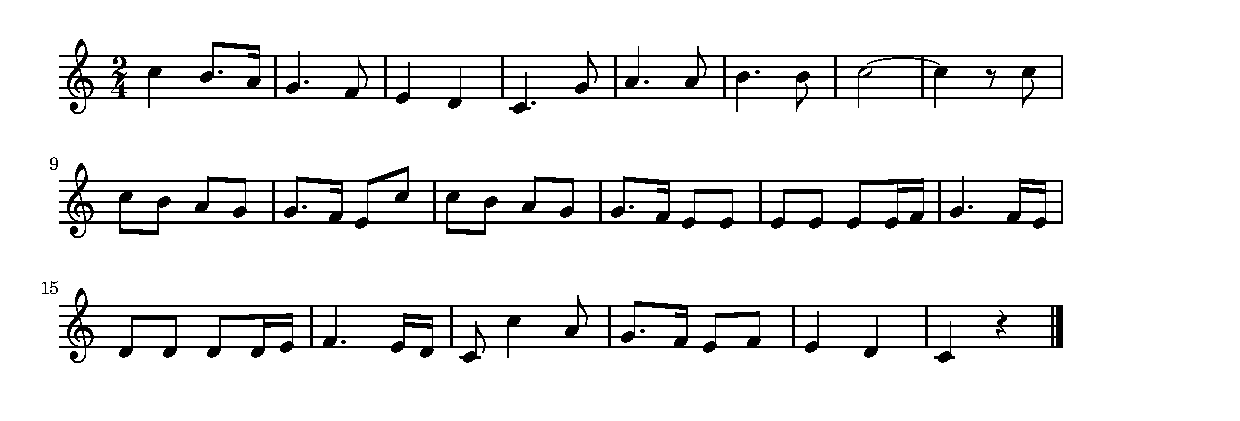
\includegraphics[clip]{morobito_crop.pdf}

\vspace{-10mm} \hspace{10mm}
もろびとこぞりて(クリスマス)
\index{もろびと@もろびとこぞりて(クリスマス)}
\index{くりすます@もろびとこぞりて(クリスマス)}

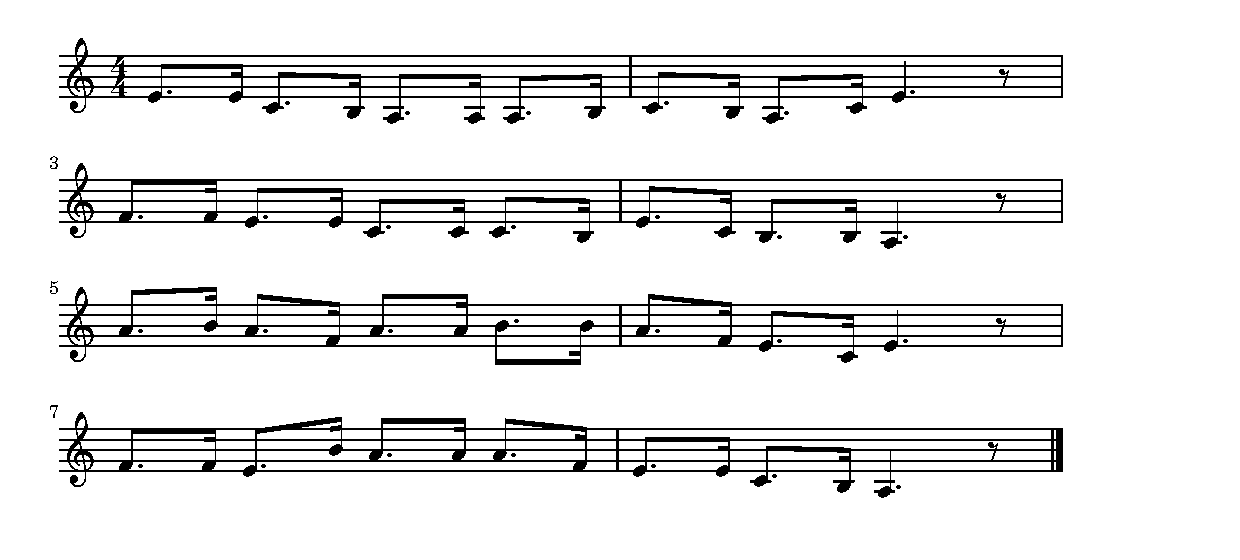
\includegraphics[clip]{nakayoshikomichi_crop.pdf}

\vspace{-10mm} \hspace{10mm}
仲よし小道(なかよしこみちはどこのみち)
\index{なかよし@仲よし小道(なかよしこみちはどこのみち)}

\includegraphics[clip]{doreminouta_crop.pdf}

\vspace{-10mm} \hspace{10mm}
ドレミの歌(どはどーなつのど)
\index{どれみのうた@ドレミの歌(どはどーなつのど)}

\includegraphics[clip]{tulip_crop.pdf}

\vspace{-10mm} \hspace{10mm}
チューリップ(さいたさいたちゅーりっぷのはなが)
\index{ちゅうりっぷ@チューリップ(さいたさいたちゅーりっぷのはなが)}

\includegraphics[clip]{kakashi_crop.pdf}

\vspace{-10mm} \hspace{10mm}
案山子(やまだのなかのいっぽんあしの)
\index{やまだ@案山子(やまだのなかのいっぽんあしの)}

\includegraphics[clip]{kagewoshitaite_crop.pdf}

\vspace{-10mm} \hspace{10mm}
影を慕いて(まぼろしのかげをしたいて)
\index{かげをしたいて@影を慕いて(まぼろしのかげをしたいて)}

\includegraphics[clip]{maritotonosama_crop.pdf}

\vspace{-10mm} \hspace{10mm}
鞠と殿さま(てんてんてんまりてんてまり)
\index{まりと@鞠と殿さま(てんてんてんまりてんてまり)}

\includegraphics[clip]{mashiroki_crop.pdf}

\vspace{-10mm} \hspace{10mm}
真白き富士の嶺(七里ヶ浜の哀歌。ましろきふじのね)
\index{ましろき@真白き富士の嶺(七里ヶ浜の哀歌。ましろきふじのね)}

\includegraphics[clip]{tennessee_crop.pdf}

\vspace{-10mm} \hspace{10mm}
テネシーワルツ
\index{てねし@テネシーワルツ}

\includegraphics[clip]{tsugaru_crop.pdf}

\vspace{-10mm} \hspace{10mm}
津軽海峡・冬景色(うえのはつのやこうれっしゃおりたときから)
\index{つがる@津軽海峡・冬景色(うえのはつのやこうれっしゃおりたときから)}

\includegraphics[clip]{sanbyaku65_crop.pdf}

\vspace{-10mm} \hspace{10mm}
三百六十五歩のマーチ(しあわせはあるいてこない)
\index{さんびゃく@三百六十五歩のマーチ(しあわせはあるいてこ}ない)

\includegraphics[clip]{wakarenoblues_crop.pdf}

\vspace{-10mm} \hspace{10mm}
別れのブルース(まどをあければ)
\index{わかれの@別れのブルース(まどをあければ)}

\includegraphics[clip]{chinatown_crop.pdf}

\vspace{-10mm} \hspace{10mm}
桑港のチャイナタウン(さんふらんしすこのちゃいなたうん)
\index{さんふらん@桑港のチャイナタウン(さんふらんしすこのちゃいなたうん)}

\includegraphics[clip]{sanpo_crop.pdf}

\vspace{-10mm} \hspace{10mm}
さんぽ(あるこうあるこうわたしはげんき)
\index{さんぽ@さんぽ(あるこうあるこうわたしはげんき)}

\includegraphics[clip]{morinokobito_crop.pdf}

\vspace{-10mm} \hspace{10mm}
森の小人(もりのこかげでどんじゃらほい)
\index{もりの@森の小人(もりのこかげでどんじゃらほい)}

\includegraphics[clip]{wakawashinouta_crop.pdf}

\vspace{-10mm} \hspace{10mm}
若鷲の歌(わかいちしおのよかれんの)
\index{わかわし@若鷲の歌(わかいちしおのよかれんの)}

\includegraphics[clip]{aranonohateni_crop.pdf}

\vspace{-10mm} \hspace{10mm}
あら野のはてに(あらののはてにゆうひはおちて。クリスマス)
\index{あらの@あら野のはてに(あらののはてにゆうひはおちて。クリスマス)}
\index{くりすます@あら野のはてに(あらののはてにゆうひはおちて。クリスマス)}

\includegraphics[clip]{awatenbo_crop.pdf}

\vspace{-10mm} \hspace{10mm}
あわてんぼうのサンタクロース(クリスマス)
\index{あわてんぼう@あわてんぼうのサンタクロース(クリスマス)}
\index{くりすます@あわてんぼうのサンタクロース(クリスマス)}

\includegraphics[clip]{makibito_crop.pdf}

\vspace{-10mm} \hspace{10mm}
牧人ひつじを(まきびとひつじをまもれる。クリスマス)
\index{まきびと@牧人ひつじを(まきびとひつじをまもれる。クリスマス)}
\index{くりすます@牧人ひつじを(まきびとひつじをまもれる。クリスマス)}

\includegraphics[clip]{fuyugeshiki_crop.pdf}

\vspace{-10mm} \hspace{10mm}
冬景色(さぎりきゆるみなとえの)
\index{ふゆげしき@冬景色(さぎりきゆるみなとえの)}

\includegraphics[clip]{hiiragi_crop.pdf}

\vspace{-10mm} \hspace{10mm}
ひいらぎかざろう(クリスマス)
\index{ひいらぎ@ひいらぎかざろう(クリスマス)}
\index{くりすます@ひいらぎかざろう(クリスマス)}

\includegraphics[clip]{nadasoso_crop.pdf}

\vspace{-10mm} \hspace{10mm}
涙そうそう(ふるいあるばむめくりありがとうってつぶやいた)
\index{なだそうそう@涙そうそう(ふるいあるばむめくりありがとうってつぶやいた)}

\includegraphics[clip]{amazinggrace_crop.pdf}

\vspace{-10mm} \hspace{10mm}
アメイジング・グレイス
\index{あめいじんぐ@アメイジング・グレイス}

\includegraphics[clip]{tsubasa_crop.pdf}

\vspace{-10mm} \hspace{10mm}
翼をください(いまわたしのねがいごとがかなうならば)
\index{つばさ@翼をください(いまわたしのねがいごとがかなうならば)}

\includegraphics[clip]{aoimewoshita_crop.pdf}

\vspace{-10mm} \hspace{10mm}
青い目の人形(あおいめをしたおにんぎょは)
\index{あおいめ@青い目の人形(あおいめをしたおにんぎょは)}

\includegraphics[clip]{aoisanmyaku_crop.pdf}

\vspace{-10mm} \hspace{10mm}
青い山脈(わかくあかるいうたごえに)
\index{あおい@青い山脈(わかくあかるいうたごえに)}

\includegraphics[clip]{uewomuite_crop.pdf}

\vspace{-10mm} \hspace{10mm}
上を向いて歩こう
\index{うえを@上を向いて歩こう}

\includegraphics[clip]{dreamisawish_crop.pdf}

\vspace{-10mm} \hspace{10mm}
夢はひそかに(ディズニー「シンデレラ」)
\index{ゆめはひそかに@夢はひそかに(ディズニー「シンデレラ」)}
\index{でぃずにー@夢はひそかに(ディズニー「シンデレラ」)}

\includegraphics[clip]{migikara2banme_crop.pdf}

\vspace{-10mm} \hspace{10mm}
右から2番目の星(ディズニー「ピーター・パン」)
\index{みぎから@右から2番目の星(ディズニー「ピーター・パン」)}
\index{でぃずにー@右から2番目の星(ディズニー「ピーター・パン」)}

\includegraphics[clip]{furusato_crop.pdf}

\vspace{-10mm} \hspace{10mm}
ふるさと(うさぎおいしかのやま)
\index{ふるさと@ふるさと(うさぎおいしかのやま)}

\includegraphics[clip]{hanawasaku_crop.pdf}

\vspace{-10mm} \hspace{10mm}
花は咲く(まっしろなゆきみちにはるかぜかおる)
\index{はなはさく@花は咲く(まっしろなゆきみちにはるかぜかおる)}

\includegraphics[clip]{hamabe_crop.pdf}

\vspace{-10mm} \hspace{10mm}
浜辺の歌(あしたはまべをさまよえば)
\index{はまべ@浜辺の歌(あしたはまべをさまよえば)}

\includegraphics[clip]{lionsleeps_crop.pdf}

\vspace{-10mm} \hspace{10mm}
ライオンは寝ている(トークンズ)
\index{らいおん@ライオンは寝ている(トークンズ)}

\includegraphics[clip]{lalalu_crop.pdf}

\vspace{-10mm} \hspace{10mm}
ラ・ラ・ルー(ディズニー「わんわん物語」)
\index{ららるー@ラ・ラ・ルー(ディズニー「わんわん物語」)}
\index{でぃずにー@ラ・ラ・ルー(ディズニー「わんわん物語」)}

\includegraphics[clip]{dragonquest_crop.pdf}

\vspace{-10mm} \hspace{10mm}
ドラゴンクエスト序曲
\index{どらごんくえすと@ドラゴンクエスト序曲}

\includegraphics[clip]{utanomachi_crop.pdf}

\vspace{-10mm} \hspace{10mm}
歌の町(よい子がすんでるよいまちは)
\index{うたのまち@歌の町(よい子がすんでるよいまちは)}

\includegraphics[clip]{shikararete_crop.pdf}

\vspace{-10mm} \hspace{10mm}
叱られて(しかられてあのこはまちまでおつかいに)
\index{しかられて@叱られて(しかられてあのこはまちまでおつかいに)}

\includegraphics[clip]{harunouta_crop.pdf}

\vspace{-10mm} \hspace{10mm}
春の唄(らららあかいはなたば)
\index{はるのうた@春の唄(らららあかいはなたば)}

\includegraphics[clip]{shonenjidai_crop.pdf}

\vspace{-10mm} \hspace{10mm}
少年時代(なつがすぎかぜあざみ)
\index{しょうねん@少年時代(なつがすぎかぜあざみ)}

\includegraphics[clip]{heighho_crop.pdf}

\vspace{-10mm} \hspace{10mm}
ハイ・ホー(くちぶえをげんきにふきならし、ディズニー「白雪姫」)
\index{はいほ@ハイ・ホー(くちぶえをげんきにふきならし、ディズニー「白雪姫」)}
\index{でぃずにー@ハイ・ホー(くちぶえをげんきにふきならし、ディズニー「白雪姫」)}

\includegraphics[clip]{syncopatedclock_crop.pdf}

\vspace{-10mm} \hspace{10mm}
シンコペーテッド・クロック(ルロイ・アンダーソン)
\index{しんこぺ@シンコペーテッド・クロック(ルロイ・アンダーソン)}

\includegraphics[clip]{honesty_crop.pdf}

\vspace{-10mm} \hspace{10mm}
オネスティ(ビリー・ジョエル)
\index{おねすてぃ@オネスティ(ビリー・ジョエル)}

\includegraphics[clip]{hinomaru_crop.pdf}

\vspace{-10mm} \hspace{10mm}
日の丸の旗(しろじにあかくひのまるそめて)
\index{ひのまる@日の丸の旗(しろじにあかくひのまるそめて)}

\includegraphics[clip]{aiai_crop.pdf}

\vspace{-10mm} \hspace{10mm}
アイアイ(あいあいあいあいおさるさんだよ)
\index{あいあいあ@アイアイ(あいあいあいあいおさるさんだよ)}

\includegraphics[clip]{bigben_crop.pdf}

\vspace{-10mm} \hspace{10mm}
ビッグ・ベンの鐘(ウェストミンスター宮殿の時計)
\index{びっぐべん@ビッグ・ベンの鐘(ウェストミンスター宮殿の時計)}

\includegraphics[clip]{lamourestbleu_crop.pdf}

\vspace{-10mm} \hspace{10mm}
恋は水色(ポール・モーリア)
\index{こいはみずいろ@恋は水色(ポール・モーリア)}

\includegraphics[clip]{kokonisachi_crop.pdf}

\vspace{-10mm} \hspace{10mm}
ここに幸あり(あらしもふけばあめもふる)
\index{ここに@ここに幸あり(あらしもふけばあめもふる)}

\includegraphics[clip]{polyrhythm_crop.pdf}

\vspace{-10mm} \hspace{10mm}
ポリリズム(Perfume とてもだいじなきみのおもいは)
\index{ぽりりずむ:ポリリズム(Perfume とてもだいじなきみのおもいは)}

\includegraphics[clip]{anomachi_crop.pdf}

\vspace{-10mm} \hspace{10mm}
あの町この町(あのまちこのまちひがくれる)
\index{あのまち@あの町この町(あのまちこのまちひがくれる)}

\includegraphics[clip]{sendo_crop.pdf}

\vspace{-10mm} \hspace{10mm}
船頭さん(むらのわたしのせんどさんは)
\index{せんど@船頭さん(むらのわたしのせんどさんは)}

\includegraphics[clip]{haruyokoimatsutoya_crop.pdf}

\vspace{-10mm} \hspace{10mm}
春よ、来い(松任谷由美。あわきひたりたつにわかあめ)
\index{はるよこい@春よ、来い(松任谷由美。あわきひたりたつにわかあめ)}

\includegraphics[clip]{takotako_crop.pdf}

\vspace{-10mm} \hspace{10mm}
たこのうた(たこたこあがれ)
\index{たこのうた@たこのうた(たこたこあがれ)}

\includegraphics[clip]{naniwabushi_crop.pdf}

\vspace{-10mm} \hspace{10mm}
浪花節だよ人生は(のめといわれてすなおにのんだ)
\index{なにわぶし@浪花節だよ人生は(のめといわれてすなおにのんだ)}

\includegraphics[clip]{maruetsu_crop.pdf}

\vspace{-10mm} \hspace{10mm}
マルエツの歌(どくたーげんきどくたーげんき)
\index{まるえつ@マルエツの歌(どくたーげんきどくたーげんき)}

\includegraphics[clip]{lawsonhyaku_crop.pdf}

\vspace{-10mm} \hspace{10mm}
ローソンストア100(ひゃくひゃくひゃくえん)
\index{ろーそん@ローソンストア100(ひゃくひゃくひゃくえん)}

\includegraphics[clip]{ksdenki_crop.pdf}

\vspace{-10mm} \hspace{10mm}
ケーズデンキの歌(ゆめゆめはっぴーいつでもやすい)
\index{けーず@ケーズデンキの歌(ゆめゆめはっぴーいつでもやすい)}

\includegraphics[clip]{sumidagawa_crop.pdf}

\vspace{-10mm} \hspace{10mm}
すみだ川(いちょうがえしにくろじゅすかけて)
\index{すみだがわ@すみだ川(いちょうがえしにくろじゅすかけて)}

\includegraphics[clip]{darekakokyowo_crop.pdf}

\vspace{-10mm} \hspace{10mm}
誰か故郷を想わざる(はなつむのべにひはおちて)
\index{だれか@誰か故郷を想わざる(はなつむのべにひはおちて)}

\includegraphics[clip]{sesamistreet_crop.pdf}

\vspace{-10mm} \hspace{10mm}
セサミストリートのテーマ(さーにーでい)
\index{せさみ@セサミストリートのテーマ(さーにーでい)}

\includegraphics[clip]{jinseigekijo_crop.pdf}

\vspace{-10mm} \hspace{10mm}
人生劇場(やるとおもえばどこまでやるさ)
\index{じんせい@人生劇場(やるとおもえばどこまでやるさ)}

\includegraphics[clip]{wakaiomawari_crop.pdf}

\vspace{-10mm} \hspace{10mm}
若いお巡りさん(もしもしべんちでささやくおふたりさん)
\index{わかい@若いお巡りさん(もしもしべんちでささやくおふたりさん)}

\includegraphics[clip]{fuyunoyoru_crop.pdf}

\vspace{-10mm} \hspace{10mm}
冬の夜(ともしびちかくきぬぬうははは)
\index{ふゆのよる@冬の夜(ともしびちかくきぬぬうははは)}

\includegraphics[clip]{usaginodance_crop.pdf}

\vspace{-10mm} \hspace{10mm}
兎のダンス(タラッタラッタラッタ)
\index{うさぎ@兎のダンス(タラッタラッタラッタ)}

\includegraphics[clip]{katyusha_crop.pdf}

\vspace{-10mm} \hspace{10mm}
カチューシャ(りんごのはなほころび)
\index{かちゅーしゃ@カチューシャ(りんごのはなほころび)}

\includegraphics[clip]{heartandsoul_crop.pdf}

\vspace{-10mm} \hspace{10mm}
ハート・アンド・ソウル(Heart and Soul)
\index{はーと@ハートアンドソウル(Heart and Soul)}

\includegraphics[clip]{sekainihitotsu_crop.pdf}

\vspace{-10mm} \hspace{10mm}
世界に一つだけの花(はなやのみせさきにならんだ)
\index{せかいにひとつ@世界に一つだけの花(はなやのみせさきにならんだ)}

\includegraphics[clip]{kokyowohanaruru_crop.pdf}

\vspace{-10mm} \hspace{10mm}
故郷を離るる歌(そののさゆりなでしこかきねのちぐさ)
\index{こきょうを@故郷を離るる歌(そののさゆりなでしこかきねのちぐさ)}

\includegraphics[clip]{amaryllis_crop.pdf}

\vspace{-10mm} \hspace{10mm}
アマリリス(みんなできこうたのしいオルゴールを)
\index{あまりりす@アマリリス(みんなできこうたのしいオルゴールを)}

\includegraphics[clip]{tokyobushi_crop.pdf}

\vspace{-10mm} \hspace{10mm}
東京節(パイノパイノパイ)
\index{とうきょうぶし@東京節(パイノパイノパイ)}

\includegraphics[clip]{korobeiniki_crop.pdf}

\vspace{-10mm} \hspace{10mm}
行商人(コロブチカ、korobeiniki, korobushka)
\index{ぎょうしょうにん@行商人(コロブチカ、korobeiniki, korobushka)}
\index{ころぶちか@行商人(コロブチカ、korobeiniki, korobushka)}

\includegraphics[clip]{haruyokoishoka_crop.pdf}

\vspace{-10mm} \hspace{10mm}
春よ来い(はるよこいはやくこいあるきはじめた)
\index{はるよこい@春よ来い(はるよこいはやくこいあるきはじめた)}

\includegraphics[clip]{kamata_crop.pdf}

\vspace{-10mm} \hspace{10mm}
蒲田行進曲(にじのみやこひかりのみなときねまのてんち)
\index{かまた@蒲田行進曲(にじのみやこひかりのみなときねまのてんち)}

\includegraphics[clip]{kalinka_crop.pdf}

\vspace{-10mm} \hspace{10mm}
カリンカ
\index{かりんか@カリンカ}

\includegraphics[clip]{duliegstmir_crop.pdf}

\vspace{-10mm} \hspace{10mm}
君は我が心の中に(Du, Du Liegst Mir Im Herzen)
\index{きみはわが@君は我が心の中に(Du, Du Liegst Mir Im Herzen)}

\includegraphics[clip]{troika_crop.pdf}

\vspace{-10mm} \hspace{10mm}
トロイカ(ゆきのしらかばなみき)
\index{とろいか@トロイカ(ゆきのしらかばなみき)}

\includegraphics[clip]{utsukushiki_crop.pdf}

\vspace{-10mm} \hspace{10mm}
美しき天然(そらにさえずるとりのこえ)
\index{うつくしき@美しき天然(そらにさえずるとりのこえ)}

\includegraphics[clip]{fuyunosonata_crop.pdf}

\vspace{-10mm} \hspace{10mm}
冬のソナタ(最初から今まで )
\index{ふゆのそなた@冬のソナタ(最初から今まで)}
\index{さいしょから@冬のソナタ(最初から今まで)}

\includegraphics[clip]{itsumonando_crop.pdf}

\vspace{-10mm} \hspace{10mm}
いつも何度でも(千と千尋の神隠し。よんでいるどこかむねのおくで)
\index{いつも@いつも何度でも(千と千尋の神隠し。よんでいるどこかむねのおくで)}

\includegraphics[clip]{shuyohitononozomino_crop.pdf}

\vspace{-10mm} \hspace{10mm}
主よ人の望みの喜びよ(J.S.バッハ)
\index{しゅよ@主よ人の望みの喜びよ(J.S.バッハ)}
\index{ばっは@主よ人の望みの喜びよ(J.S.バッハ)}

\includegraphics[clip]{letitgointro_crop.pdf}

\vspace{-10mm} \hspace{10mm}
ありのままで(アナと雪の女王イントロ。let It Go)
\index{ありのままで@ありのままで(アナと雪の女王イントロ。let It Go)}

\includegraphics[clip]{masu_crop.pdf}

\vspace{-10mm} \hspace{10mm}
ます(シューベルト)
\index{ます@ます(シューベルト)}
\index{しゅーべると@ます(シューベルト)}

\includegraphics[clip]{kareinaru_crop.pdf}

\vspace{-10mm} \hspace{10mm}
華麗なる大円舞曲(ショパン)
\index{かれいなる@華麗なる大円舞曲(ショパン)}
\index{しょぱん@華麗なる大円舞曲(ショパン)}

\includegraphics[clip]{tengokujigoku_crop.pdf}

\vspace{-10mm} \hspace{10mm}
天国と地獄(オッフェンバック)
\index{てんごく@天国と地獄(オッフェンバック)}

\includegraphics[clip]{csikospost_crop.pdf}

\vspace{-10mm} \hspace{10mm}
クシコス・ポスト(ネッケ)
\index{くしこす@クシコス・ポスト(ネッケ)}

\includegraphics[clip]{gunkan_crop.pdf}

\vspace{-10mm} \hspace{10mm}
軍艦マーチ(まもるもせむるも)
\index{ぐんかん@軍艦マーチ(まもるもせむるも)}

\includegraphics[clip]{koitowadonna_crop.pdf}

\vspace{-10mm} \hspace{10mm}
恋とはどんなものかしら(モーツアルト。フィガロの結婚より)
\index{こいとは@恋とはどんなものかしら(モーツアルト。フィガロの結婚より)}
\index{もーつぁると@恋とはどんなものかしら(モーツアルト。フィガロの結婚より)}

\includegraphics[clip]{doukinosakura_crop.pdf}

\vspace{-10mm} \hspace{10mm}
同期の桜(きさまとおれとは)
\index{どうき@同期の桜(きさまとおれとは)}

\includegraphics[clip]{tokyoondo_crop.pdf}

\vspace{-10mm} \hspace{10mm}
東京音頭(とうきょうおんど。はあーおどりおどるならちょいと)
\index{とうきょう@東京音頭(とうきょうおんど。はあーおどりおどるならちょいと)}

\includegraphics[clip]{gymnopedies_crop.pdf}

\vspace{-10mm} \hspace{10mm}
ジムノペディ1番(サティ)
\index{じむ@ジムノペディ1番(サティ)}
\index{さてぃ@ジムノペディ1番(サティ)}

\includegraphics[clip]{amairodebussy_crop.pdf}

\vspace{-10mm} \hspace{10mm}
亜麻色の髪の乙女(ドビュッシー)
\index{あまいろ@亜麻色の髪の乙女(ドビュッシー)}
\index{どびゅっしー@亜麻色の髪の乙女(ドビュッシー)}

\includegraphics[clip]{donau_crop.pdf}

\vspace{-10mm} \hspace{10mm}
美しき青きドナウ(ヨハン・シュトラウス2世)
\index{うつくしき@美しき青きドナウ(ヨハン・シュトラウス2世)}

\includegraphics[clip]{jeteveux_crop.pdf}

\vspace{-10mm} \hspace{10mm}
ジュ・トゥ・ヴ(エリック・サティ)
\index{じゅとぶ@ジュ・トゥ・ヴ(エリック・サティ)}
\index{さてぃ@ジュ・トゥ・ヴ(エリック・サティ)}

\includegraphics[clip]{mozartkomori_crop.pdf}

\vspace{-10mm} \hspace{10mm}
モーツァルトの子守歌
\index{もーつ@モーツァルトの子守歌}
\index{こもりうた@モーツァルトの子守歌}

\includegraphics[clip]{brahmskomori_crop.pdf}

\vspace{-10mm} \hspace{10mm}
ブラームスの子守歌
\index{ぶらーむす@ブラームスの子守歌}
\index{こもりうた@ブラームスの子守歌}

\includegraphics[clip]{unmei_crop.pdf}

\vspace{-10mm} \hspace{10mm}
運命(ベートーベン交響曲5番)
\index{うんめい@運命(ベートーベン交響曲5番)}

\includegraphics[clip]{habanera_crop.pdf}

\vspace{-10mm} \hspace{10mm}
ハバネラ(ビゼー。カルメンより)
\index{はばねら@ハバネラ(ビゼー。カルメンより)}

\includegraphics[clip]{shinsekai_crop.pdf}

\vspace{-10mm} \hspace{10mm}
新世界(ドヴォルザーク)
\index{しんせかい@新世界(ドヴォルザーク)}

\includegraphics[clip]{vivaldishiki_crop.pdf}

\vspace{-10mm} \hspace{10mm}
ヴィヴァルディ四季より春
\index{ゔぃゔぁるでぃ@ヴィヴァルディ四季より春}

\includegraphics[clip]{ifudodo_crop.pdf}

\vspace{-10mm} \hspace{10mm}
威風堂々(エルガー)
\index{いふうどうどう@威風堂々(エルガー)}

\includegraphics[clip]{mendelsharunouta_crop.pdf}

\vspace{-10mm} \hspace{10mm}
春の歌(メンデルスゾーン)
\index{はるのうた@春の歌(メンデルスゾーン)}

\includegraphics[clip]{kanpai_crop.pdf}

\vspace{-10mm} \hspace{10mm}
乾杯の歌(ヴェルディ)
\index{かんぱい@乾杯の歌(ヴェルディ)}

\includegraphics[clip]{radetzky_crop.pdf}

\vspace{-10mm} \hspace{10mm}
ラデツキー行進曲(ヨハン・シュトラウス1世)
\index{らでつきー@ラデツキー行進曲(ヨハン・シュトラウス1世)}

\includegraphics[clip]{zuizui_crop.pdf}

\vspace{-10mm} \hspace{10mm}
ずいずいずっころばし
\index{ずいずい@ずいずいずっころばし}

\includegraphics[clip]{moeroyo_crop.pdf}

\vspace{-10mm} \hspace{10mm}
燃えろよ燃えろよ
\index{もえろよ@燃えろよ燃えろよ}

\includegraphics[clip]{mybonnie_crop.pdf}

\vspace{-10mm} \hspace{10mm}
マイボニー(My Bonnie Lies Over the Ocean)
\index{まいぼにー@マイボニー(My Bonnie Lies Over the Ocean)}

\includegraphics[clip]{chairo_crop.pdf}

\vspace{-10mm} \hspace{10mm}
茶色の小瓶
\index{ちゃいろの@茶色の小瓶}

\includegraphics[clip]{gonbe_crop.pdf}

\vspace{-10mm} \hspace{10mm}
権兵衛さんの赤ちゃん(ごんべえさんのあかちゃんが)
\index{ごんべえ@権兵衛さんの赤ちゃん(ごんべえさんのあかちゃんが)}

\includegraphics[clip]{yamanoongakuka_crop.pdf}

\vspace{-10mm} \hspace{10mm}
山の音楽家(わたしゃおんがくかやまのこりす)
\index{やまのおんがくか@山の音楽家(わたしゃおんがくかやまのこりす)}

\includegraphics[clip]{mokusei_crop.pdf}

\vspace{-10mm} \hspace{10mm}
木星(ホルスト「惑星」よりジュピター)
\index{もくせい@木星(ホルスト「惑星」よりジュピター)}

\includegraphics[clip]{eineclinenacht_crop.pdf}

\vspace{-10mm} \hspace{10mm}
アイネ・クライネ・ナハト・ムジーク(モーツァルト)
\index{あいねくらいね@アイネ・クライネ・ナハト・ムジーク(モーツァルト)}

\includegraphics[clip]{amadare_crop.pdf}

\vspace{-10mm} \hspace{10mm}
雨だれの前奏曲(ショパン)
\index{あまだれ@雨だれの前奏曲(ショパン)}

\includegraphics[clip]{ainoyorokobi_crop.pdf}

\vspace{-10mm} \hspace{10mm}
愛の喜び(マルティーニ)
\index{あいのよろこび@愛の喜び(マルティーニ)}

\includegraphics[clip]{edokomori_crop.pdf}

\vspace{-10mm} \hspace{10mm}
江戸の子守唄(ねんねんころりよおころりよ)
\index{えど@江戸の子守唄(ねんねんころりよおころりよ)}
\index{こもりうた@江戸の子守唄(ねんねんころりよおころりよ)}

\includegraphics[clip]{antagata_crop.pdf}

\vspace{-10mm} \hspace{10mm}
あんたがたどこさ(ひごさひごどこさくまもとさ)
\index{あんたがた@あんたがたどこさ(ひごさひごどこさくまもとさ)}

\includegraphics[clip]{isshukan_crop.pdf}

\vspace{-10mm} \hspace{10mm}
一週間(にちようびにいちばにでかけ)
\index{いっしゅうかん@一週間(にちようびにいちばにでかけ)}

\includegraphics[clip]{morinokuma_crop.pdf}

\vspace{-10mm} \hspace{10mm}
森のくまさん(あるひもりのなかくまさんにであった)
\index{もり@森のくまさん(あるひもりのなかくまさんにであった)}

\includegraphics[clip]{kawanonagare_crop.pdf}

\vspace{-10mm} \hspace{10mm}
川の流れのように(しらずしらずあるいてきた)
\index{かわ@川の流れのように(しらずしらずあるいてきた)}

\includegraphics[clip]{natsunoomoide_crop.pdf}

\vspace{-10mm} \hspace{10mm}
夏の思い出(なつがくればおもいだす)
\index{なつ@夏の思い出(なつがくればおもいだす)}

\includegraphics[clip]{waltzbrahms_crop.pdf}

\vspace{-10mm} \hspace{10mm}
ブラームスのワルツ(円舞曲)
\index{ぶら@ブラームスのワルツ(円舞曲)}

\includegraphics[clip]{senrowa_crop.pdf}

\vspace{-10mm} \hspace{10mm}
線路は続くよどこまでも(せんろはつづくよどこまでも)
\index{せんろ@線路は続くよどこまでも(せんろはつづくよどこまでも)}

\includegraphics[clip]{shiawasenara_crop.pdf}

\vspace{-10mm} \hspace{10mm}
幸せなら手をたたこう(しあわせならてをたたこう)
\index{しあわせ@幸せなら手をたたこう(しあわせならてをたたこう)}


\includegraphics[clip]{yukiyakonko_crop.pdf}

\vspace{-10mm} \hspace{10mm}
雪(ゆきやこんこあられやこんこ)
\index{ゆき@雪(ゆきやこんこあられやこんこ)}

\includegraphics[clip]{kitaguninoharu_crop.pdf}

\vspace{-10mm} \hspace{10mm}
北国の春(しらかばあおぞらみなみかぜ)
\index{きたぐに@北国の春(しらかばあおぞらみなみかぜ)}

\includegraphics[clip]{shizukanakohan_crop.pdf}

\vspace{-10mm} \hspace{10mm}
静かな湖畔(しずかなこはんのもりのかげから)
\index{しずか@静かな湖畔(しずかなこはんのもりのかげから)}

\includegraphics[clip]{onnanomichi_crop.pdf}

\vspace{-10mm} \hspace{10mm}
女のみち(わたしがささげたそのひとに)
\index{おんな@女のみち(わたしがささげたそのひとに)}


\includegraphics[clip]{omochanochachacha_crop.pdf}

\vspace{-10mm} \hspace{10mm}
おもちゃのチャチャチャ
\index{おもちゃの@おもちゃのチャチャチャ}

\includegraphics[clip]{peergyntasagrieg_crop.pdf}

\vspace{-10mm} \hspace{10mm}
ペールギュントより朝(グリーグ)
\index{ぺーる@ペールギュントより朝(グリーグ)}

\includegraphics[clip]{hornmozart_crop.pdf}

\vspace{-10mm} \hspace{10mm}
ホルン協奏曲第1番(モーツァルト)
\index{ほるん@ホルン協奏曲第1番(モーツァルト)}

\includegraphics[clip]{ikenoame_crop.pdf}

\vspace{-10mm} \hspace{10mm}
池の雨(ヤマハ音楽教室幼児科メロディー暗唱曲)
\index{いけ@池の雨(ヤマハ音楽教室幼児科メロディー暗唱曲)}

\includegraphics[clip]{turkbeethoven_crop.pdf}

\vspace{-10mm} \hspace{10mm}
ベートーベンのトルコ行進曲
\index{べーと@ベートーベンのトルコ行進曲}
\index{とるこ@ベートーベンのトルコ行進曲}

\includegraphics[clip]{genkotsu_crop.pdf}

\vspace{-10mm} \hspace{10mm}
げんこつやまのたぬきさん
\index{げんこつやまの@げんこつやまのたぬきさん}

\includegraphics[clip]{seija_crop.pdf}

\vspace{-10mm} \hspace{10mm}
聖者が街にやってくる(聖者の行進))
\index{せいじゃ@聖者が街にやってくる(聖者の行進))}

\includegraphics[clip]{kogitsune_crop.pdf}

\vspace{-10mm} \hspace{10mm}
こぎつね(こぎつねこんこんやまのなか)
\index{こぎつね@こぎつね(こぎつねこんこんやまのなか)}

\includegraphics[clip]{londonbashi_crop.pdf}

\vspace{-10mm} \hspace{10mm}
ロンドン橋(ろんどんばしおちた)
\index{ろんどん@ロンドン橋(ろんどんばしおちた)}

\includegraphics[clip]{marysanno_crop.pdf}

\vspace{-10mm} \hspace{10mm}
メリーさんの羊(めりーさんのひつじ)
\index{めりー@メリーさんの羊(めりーさんのひつじ)}

\includegraphics[clip]{abrahamunoko_crop.pdf}

\vspace{-10mm} \hspace{10mm}
アブラハムの子(あぶらはむにはしちにんのこ)
\index{あぶらはむ@アブラハムの子(あぶらはむにはしちにんのこ)}

\includegraphics[clip]{chatsumi_crop.pdf}

\vspace{-10mm} \hspace{10mm}
茶摘(ちゃつみ。なつもちかづくはちじゅうはちや)
\index{@茶摘(ちゃつみ。なつもちかづくはちじゅうはちや)}

\includegraphics[clip]{okinafurudokei_crop.pdf}

\vspace{-10mm} \hspace{10mm}
大きな古時計(おおきなのっぽのふるどけい)
\index{おおきなふる@大きな古時計(おおきなのっぽのふるどけい)}

\includegraphics[clip]{takibi_crop.pdf}

\vspace{-10mm} \hspace{10mm}
たき火(かきねのかきねのまがりかど)
\index{たきび@たき火(かきねのかきねのまがりかど)}

\includegraphics[clip]{shikinouta_crop.pdf}

\vspace{-10mm} \hspace{10mm}
四季の歌(はるをあいするひとは)
\index{しきの@四季の歌(はるをあいするひとは)}

\includegraphics[clip]{katatsumuri_crop.pdf}

\vspace{-10mm} \hspace{10mm}
かたつむり(でんでんむしむし)
\index{かたつむり@かたつむり(でんでんむしむし)}

\includegraphics[clip]{hotarukoi_crop.pdf}

\vspace{-10mm} \hspace{10mm}
ほたるこい
\index{ほたるこい@ほたるこい}

\includegraphics[clip]{kagome_crop.pdf}

\vspace{-10mm} \hspace{10mm}
かごめかごめ(かごのなかのとりは)
\index{かごめ@かごめかごめ(かごのなかのとりは)}

\includegraphics[clip]{kaerunogassho_crop.pdf}

\vspace{-10mm} \hspace{10mm}
かえるの合唱(かえるのうたがきこえてくるよ)
\index{かえる@かえるの合唱(かえるのうたがきこえてくるよ)}

\includegraphics[clip]{yukainamakiba_crop.pdf}

\vspace{-10mm} \hspace{10mm}
ゆかいな牧場(いちろうさんのまきばでいーあいいーあいおー)
\index{ゆかいな@ゆかいな牧場(いちろうさんのまきばでいーあいいーあいおー)}

\includegraphics[clip]{bunbunbun_crop.pdf}

\vspace{-10mm} \hspace{10mm}
ぶんぶんぶん(ぶんぶんぶんはちがとぶ)
\index{ぶんぶんぶん@ぶんぶんぶん(ぶんぶんぶんはちがとぶ)}

\includegraphics[clip]{okinakuri_crop.pdf}

\vspace{-10mm} \hspace{10mm}
大きな栗の木の下で(おおきなくりのきのしたで)
\index{おおきなくり@大きな栗の木の下で(おおきなくりのきのしたで)}

\includegraphics[clip]{tonbono_crop.pdf}

\vspace{-10mm} \hspace{10mm}
とんぼのめがね
\index{とんぼの@とんぼのめがね}

\includegraphics[clip]{oshogatsu_crop.pdf}

\vspace{-10mm} \hspace{10mm}
お正月(もういくつねるとおしょうがつ)
\index{おしょうがつ@お正月(もういくつねるとおしょうがつ)}

\includegraphics[clip]{tewotata_crop.pdf}

\vspace{-10mm} \hspace{10mm}
手をたたきましょう
\index{てをたたき@手をたたきましょう}

\includegraphics[clip]{gaisen_crop.pdf}

\vspace{-10mm} \hspace{10mm}
凱旋行進曲(ヴェルディ。アイーダ)
\index{がいせん@凱旋行進曲(ヴェルディ。アイーダ)}

\includegraphics[clip]{obladi_crop.pdf}

\vspace{-10mm} \hspace{10mm}
Ob-La-Di, Ob-La-Da (ビートルズ)
\index{おぶらでぃ@Ob-La-Di, Ob-La-Da (ビートルズ)}

\includegraphics[clip]{carrythatweight_crop.pdf}

\vspace{-10mm} \hspace{10mm}
Carry That Weight (ビートルズ)
\index{きゃりーざっと@Carry That Weight (ビートルズ)}

\includegraphics[clip]{acrossuniverse_crop.pdf}

\vspace{-10mm} \hspace{10mm}
Across the Universe (ビートルズ)
\index{あくろす@Across the Universe (ビートルズ)}

\includegraphics[clip]{yurakucho_crop.pdf}

\vspace{-10mm} \hspace{10mm}
有楽町で逢いましょう(あなたをまてばあめがふる)
\index{ゆうらくちょう@有楽町で逢いましょう(あなたをまてばあめがふる)}

\includegraphics[clip]{cosmos_crop.pdf}

\vspace{-10mm} \hspace{10mm}
秋桜(うすべにのこすもすがあきのひの)
\index{こすもす@秋桜(うすべにのこすもすがあきのひの)}

\includegraphics[clip]{dango3kyodai_crop.pdf}

\vspace{-10mm} \hspace{10mm}
だんご3兄弟(くしにささってだんごだんご)
\index{だんごさん@だんご3兄弟(くしにささってだんごだんご)}

\includegraphics[clip]{chimchimcheree_crop.pdf}

\vspace{-10mm} \hspace{10mm}
チム・チム・チェリー(ちむちむにーちむちむにー)
\index{ちむちむちぇりー@チム・チム・チェリー(ちむちむにーちむちむにー)}

\includegraphics[clip]{tetsuwan_crop.pdf}

\vspace{-10mm} \hspace{10mm}
鉄腕アトム(そらをこえてららら)
\index{てつわんあとむ@鉄腕アトム(そらをこえてららら)}

\includegraphics[clip]{yogiriyo_crop.pdf}

\vspace{-10mm} \hspace{10mm}
夜霧よ今夜もありがとう(しのびあうこいをつつむよぎりよ)
\index{よぎりよ@夜霧よ今夜もありがとう(しのびあうこいをつつむよぎりよ)}


\includegraphics[clip]{hoshinonagareni_crop.pdf}

\vspace{-10mm} \hspace{10mm}
星の流れに(ほしのながれにみをうらなって)
\index{ほしのながれに@星の流れに(ほしのながれにみをうらなって)}



\includegraphics[clip]{ichigatsuichijitsu_crop.pdf}

\vspace{-10mm} \hspace{10mm}
一月一日(いちがついちじつ、としのはじめのためしとて)
\index{いちがつ@一月一日(いちがついちじつ、としのはじめのためしとて)}



\includegraphics[clip]{kakkou_crop.pdf}

\vspace{-10mm} \hspace{10mm}
かっこう
\index{かっこう}



\includegraphics[clip]{kirakira_crop.pdf}

\vspace{-10mm} \hspace{10mm}
きらきら星(きらきらぼし)
\index{きらきら@きらきら星(きらきらぼし)}



\includegraphics[clip]{koinobori_crop.pdf}

\vspace{-10mm} \hspace{10mm}
こいのぼり(やねよりたかい)
\index{こいのぼり(やねよりたかい)}



\includegraphics[clip]{konomichi_crop.pdf}

\vspace{-10mm} \hspace{10mm}
この道(このみちはいつかきたみち)
\index{このみち@この道(このみちはいつかきたみち)}



\includegraphics[clip]{konoyonohana_crop.pdf}

\vspace{-10mm} \hspace{10mm}
この世の花(このよのはな。あかくさくはなあおいはな)
\index{このよの@この世の花(このよのはな。あかくさくはなあおいはな)}



\includegraphics[clip]{mickeymousemarch_crop.pdf}

\vspace{-10mm} \hspace{10mm}
ミッキーマウス・マーチ(ぼくらのくらぶのりーだーは)
\index{みっきーまうす@ミッキーマウス・マーチ(ぼくらのくらぶのりーだーは)}


\includegraphics[clip]{mikan_crop.pdf}

\vspace{-10mm} \hspace{10mm}
みかんの花咲く丘(みかんのはながさいている)
\index{みかんの@みかんの花咲く丘(みかんのはながさいている)}



\includegraphics[clip]{momiji_crop.pdf}

\vspace{-10mm} \hspace{10mm}
もみじ(あきのゆうひにてるやま)
\index{もみじ(あきのゆうひにてるやま)}



\includegraphics[clip]{mushinokoe_crop.pdf}

\vspace{-10mm} \hspace{10mm}
虫の声(あれまつむしがないている)
\index{むしのこえ@虫の声(あれまつむしがないている)}



\includegraphics[clip]{musunde_crop.pdf}

\vspace{-10mm} \hspace{10mm}
むすんでひらいて(むすんでひらいててをうってむすんで)
\index{むすんでひらいて(むすんでひらいててをうってむすんで)}



\includegraphics[clip]{nangoku_crop.pdf}

\vspace{-10mm} \hspace{10mm}
南国土佐を後にして(なんごくとさをあとにして)
\index{なんごくとさ@南国土佐を後にして(なんごくとさをあとにして)}





\includegraphics[clip]{onetwojenkka_crop.pdf}

\vspace{-10mm} \hspace{10mm}
ワンツー・ジェンカ(おおきくくちあけて)
\index{わんつーじぇんか@ワンツー・ジェンカ(おおきくくちあけて)}


\includegraphics[clip]{saikai_crop.pdf}

\vspace{-10mm} \hspace{10mm}
再会(さいかい。あえなくなってはじめてしった)
\index{さいかい@再会(さいかい。あえなくなってはじめてしった)}



\includegraphics[clip]{sakura_crop.pdf}

\vspace{-10mm} \hspace{10mm}
さくらさくら
\index{さくらさくら}



\includegraphics[clip]{shuchou_crop.pdf}

\vspace{-10mm} \hspace{10mm}
酋長の娘(わたしのらばさん)
\index{しゅうちょう@酋長の娘(わたしのらばさん)}




\includegraphics[clip]{smallworld_crop.pdf}

\vspace{-10mm} \hspace{10mm}
小さな世界(ちいさなせかい、It's a small world、せかいじゅうどこだって)
\index{ちいさなせかい@小さな世界(ちいさなせかい、It's a small world、せかいじゅうどこだって)}



\includegraphics[clip]{takedanokomori_crop.pdf}

\vspace{-10mm} \hspace{10mm}
竹田の子もりうた(もりもいやがるぼんから)
\index{たけだのこもり@竹田の子もりうた(もりもいやがるぼんから)}



\includegraphics[clip]{tonakai_crop.pdf}

\vspace{-10mm} \hspace{10mm}
赤鼻のトナカイ(Rudolph the Red-Nosed Reindeer、まっかなおはなの。クリスマス)
\index{あかはなの@赤鼻のトナカイ(Rudolph the Red-Nosed Reindeer、まっかなおはなの。クリスマス)}
\index{くりすます@赤鼻のトナカイ(Rudolph the Red-Nosed Reindeer、まっかなおはなの。クリスマス)}



\includegraphics[clip]{gensou_crop.pdf}

\vspace{-10mm} \hspace{10mm}
幻想即興曲(ショパン)
\index{げんそうそっきょうきょく@幻想即興曲(ショパン)}

\includegraphics[clip]{kimigayo_crop.pdf}

\vspace{-10mm} \hspace{10mm}
君が代(きみがよはちよにやちよに)
\index{きみがよ@君が代(きみがよはちよにやちよに)}

\includegraphics[clip]{schubertkomori_crop.pdf}

\vspace{-10mm} \hspace{10mm}
シューベルトの子守歌(ねむれねむらははのむねに)
\index{しゅーべると@シューベルトの子守歌(ねむれねむらははのむねに)}
\index{こもりうた@シューベルトの子守歌(ねむれねむらははのむねに)}

\includegraphics[clip]{schubertnobara_crop.pdf}

\vspace{-10mm} \hspace{10mm}
シューベルトの野ばら(わらべはみたりのなかのばら)
\index{しゅーべるとののばら@シューベルトの野ばら(わらべはみたりのなかのばら)}

\includegraphics[clip]{yakyuken_crop.pdf}

\vspace{-10mm} \hspace{10mm}
野球拳(やきゅうけん。やきゅうするならこういうぐあいにしやしゃんせ)
\index{やきゅうけん@野球拳(やきゅうけん。やきゅうするならこういうぐあいにしやしゃんせ)}

\includegraphics[clip]{akaikutsu_crop.pdf}

\vspace{-10mm} \hspace{10mm}
赤い靴(あかいくつはいてたおんなのこ)
\index{あかいくつ@赤い靴(あかいくつはいてたおんなのこ)}

\includegraphics[clip]{akatonbo_crop.pdf}

\vspace{-10mm} \hspace{10mm}
赤とんぼ(ゆうやけこやけのあかとんぼ)
\index{あかとんぼ@赤とんぼ(ゆうやけこやけのあかとんぼ)}

\includegraphics[clip]{amaironokami_crop.pdf}

\vspace{-10mm} \hspace{10mm}
亜麻色の髪の乙女(ヴィレッジ・シンガーズ。あまいろのながいかみをかぜが)
\index{あまいろの@亜麻色の髪の乙女(あまいろのながいかみをかぜが)}

\includegraphics[clip]{anokowatare_crop.pdf}

\vspace{-10mm} \hspace{10mm}
あの子はたあれ(あのこはたあれたれでしょね)
\index{あのこは@あの子はたあれ(あのこはたあれたれでしょね)}

\includegraphics[clip]{aogeba_crop.pdf}

\vspace{-10mm} \hspace{10mm}
仰げば尊し(あおげばとうとしわがしのおん)
\index{あおげば@仰げば尊し(あおげばとうとしわがしのおん)}

\includegraphics[clip]{chouchou_crop.pdf}

\vspace{-10mm} \hspace{10mm}
ちょうちょう(ちょうちょうちょうちょうなのはにとまれ)
\index{ちょうちょう(ちょうちょうちょうちょうなのはにとまれ)}

\includegraphics[clip]{countryroad_crop.pdf}

\vspace{-10mm} \hspace{10mm}
カントリー・ロード(かんとりーろーど、このみち)
\index{かんとりー@カントリー・ロード(かんとりーろーど、このみち)}

\includegraphics[clip]{donguri_crop.pdf}

\vspace{-10mm} \hspace{10mm}
どんぐりころころ(どんぐりころころどんぶりこ)
\index{どんぐりころころ(どんぐりころころどんぶりこ)}

\includegraphics[clip]{fujisan_crop.pdf}

\vspace{-10mm} \hspace{10mm}
富士山(ふじさん。あたまをくものうえにだし)
\index{ふじさん@富士山(ふじさん。あたまをくものうえにだし)}

\includegraphics[clip]{harugakita_crop.pdf}

\vspace{-10mm} \hspace{10mm}
春が来た(はるがきた)
\index{はるがきた@春が来た(はるがきた)}

\includegraphics[clip]{harukaze_crop.pdf}

\vspace{-10mm} \hspace{10mm}
春風(ふけそよそよふけはるかぜよ)
\index{はるかぜ@春風(ふけそよそよふけはるかぜよ)}

\includegraphics[clip]{harunoogawa_crop.pdf}

\vspace{-10mm} \hspace{10mm}
春の小川(はるのおがわはさらさらながる)
\index{はるのおがわ@春の小川(はるのおがわはさらさらながる)}


\includegraphics[clip]{usagi_crop.pdf}

\vspace{-10mm} \hspace{10mm}
うさぎ(うさぎうさぎなにみてはねる)
\index{うさぎ(うさぎうさぎなにみてはねる)}

\includegraphics[clip]{warewaumi_crop.pdf}

\vspace{-10mm} \hspace{10mm}
われは海の子(われはうみのこしらなみの)
\index{われはうみのこ@われは海の子(われはうみのこしらなみの)}

\includegraphics[clip]{yashinomi_crop.pdf}

\vspace{-10mm} \hspace{10mm}
椰子の実(やしのみ。なもしらぬとおきしまより)
\index{やしのみ@椰子の実(やしのみ。なもしらぬとおきしまより)}

\includegraphics[clip]{yesterdayonce_crop.pdf}

\vspace{-10mm} \hspace{10mm}
イエスタデイ・ワンス・モア(カーペンターズ)
\index{いえすたでいわんす@イエスタデイ・ワンス・モア(カーペンターズ)}

\includegraphics[clip]{yuki100p_crop.pdf}

\vspace{-10mm} \hspace{10mm}
勇気100パーセント(がっかりしてめそめそしてどうしたんだい)
\index{ゆうきひゃくぱーせんと@勇気100パーセント(がっかりしてめそめそしてどうしたんだい)}

\includegraphics[clip]{yorokobi_crop.pdf}

\vspace{-10mm} \hspace{10mm}
喜びの歌(はれたるあおぞらただようくもよ)
\index{よろこびのうた@喜びの歌(はれたるあおぞらただようくもよ)}

\newpage
\printindex

\end{document}
